\documentclass{beamer}\usepackage[]{graphicx}\usepackage[]{color}
%% maxwidth is the original width if it is less than linewidth
%% otherwise use linewidth (to make sure the graphics do not exceed the margin)
\makeatletter
\def\maxwidth{ %
  \ifdim\Gin@nat@width>\linewidth
    \linewidth
  \else
    \Gin@nat@width
  \fi
}
\makeatother

\definecolor{fgcolor}{rgb}{0.345, 0.345, 0.345}
\newcommand{\hlnum}[1]{\textcolor[rgb]{0.686,0.059,0.569}{#1}}%
\newcommand{\hlstr}[1]{\textcolor[rgb]{0.192,0.494,0.8}{#1}}%
\newcommand{\hlcom}[1]{\textcolor[rgb]{0.678,0.584,0.686}{\textit{#1}}}%
\newcommand{\hlopt}[1]{\textcolor[rgb]{0,0,0}{#1}}%
\newcommand{\hlstd}[1]{\textcolor[rgb]{0.345,0.345,0.345}{#1}}%
\newcommand{\hlkwa}[1]{\textcolor[rgb]{0.161,0.373,0.58}{\textbf{#1}}}%
\newcommand{\hlkwb}[1]{\textcolor[rgb]{0.69,0.353,0.396}{#1}}%
\newcommand{\hlkwc}[1]{\textcolor[rgb]{0.333,0.667,0.333}{#1}}%
\newcommand{\hlkwd}[1]{\textcolor[rgb]{0.737,0.353,0.396}{\textbf{#1}}}%
\let\hlipl\hlkwb

\usepackage{framed}
\makeatletter
\newenvironment{kframe}{%
 \def\at@end@of@kframe{}%
 \ifinner\ifhmode%
  \def\at@end@of@kframe{\end{minipage}}%
  \begin{minipage}{\columnwidth}%
 \fi\fi%
 \def\FrameCommand##1{\hskip\@totalleftmargin \hskip-\fboxsep
 \colorbox{shadecolor}{##1}\hskip-\fboxsep
     % There is no \\@totalrightmargin, so:
     \hskip-\linewidth \hskip-\@totalleftmargin \hskip\columnwidth}%
 \MakeFramed {\advance\hsize-\width
   \@totalleftmargin\z@ \linewidth\hsize
   \@setminipage}}%
 {\par\unskip\endMakeFramed%
 \at@end@of@kframe}
\makeatother

\definecolor{shadecolor}{rgb}{.97, .97, .97}
\definecolor{messagecolor}{rgb}{0, 0, 0}
\definecolor{warningcolor}{rgb}{1, 0, 1}
\definecolor{errorcolor}{rgb}{1, 0, 0}
\newenvironment{knitrout}{}{} % an empty environment to be redefined in TeX

\usepackage{alltt}
\usetheme{default}
%\usetheme{Malmoe}

\title[EC999: Quantitative Text Analysis]{EC999: Introduction} \def\newblock{\hskip .11em plus .33em minus .07em}


\def\Tiny{\fontsize{10pt}{10pt}\selectfont}
\def\smaller{\fontsize{8pt}{8pt}\selectfont}

\institute[Warwick]{University of Chicago \& University of Warwick}
\author[Thiemo Fetzer]{Thiemo Fetzer}

 \date{\today}

\usepackage{natbib}
\usepackage{amsmath}
\usepackage{hyperref}
\usepackage{graphicx}
\usepackage{graphics}

\usepackage{amsfonts}
\usepackage{amssymb}
\usepackage{pdfpages}
\usepackage{natbib}
\usepackage{hyperref}
%\usepackage{enumitem}
 \usepackage{pgffor}
\usepackage{booktabs,caption,fixltx2e}
\usepackage[flushleft]{threeparttable}
\usepackage{verbatim} 
\usepackage{cancel}
\newcommand\xxcancel[1]{\xcancel{#1}\vphantom{#1}}

\usepackage{mathtools,xparse}

\newenvironment{Description}
               {\list{}{\labelwidth=0pt \itemindent-\leftmargin
                        \let\makelabel\Descriptionlabel
                        % or whatever
               }}
               {\endlist}
\newcommand*\Descriptionlabel[1]{%
  \hspace\labelsep
  \normalfont%  reset current font setting
  \color{blue}\bfseries\sffamily% or whatever 
  #1}


\setbeamersize{text margin left = 16pt, text margin right = 16pt}
\newcommand{\code}[1]{\texttt{#1}}

\newenvironment<>{algorithm}[1][\undefined]{%
\begin{actionenv}#2%
\ifx#1\undefined%
   \def\insertblocktitle{Algorithm}%
\else%
   \def\insertblocktitle{Algorithm ({\em#1})}%
\fi%
\par%
\mode<presentation>{%
  \setbeamercolor{block title}{fg=white,bg=yellow!50!black}
  \setbeamercolor{block body}{fg=black,bg=yellow!20}
}%
\usebeamertemplate{block begin}\em}
{\par\usebeamertemplate{block end}\end{actionenv}}


\newenvironment<>{assumption}[1][\undefined]{%
\begin{actionenv}#2%
\ifx#1\undefined%
   \def\insertblocktitle{Assumption}%
\else%
   \def\insertblocktitle{Assumption ({\em#1})}%
\fi%
\par%
\mode<presentation>{%
  \setbeamercolor{block title}{fg=white,bg=blue!50!black}
  \setbeamercolor{block body}{fg=black,bg=blue!20}
}%
\usebeamertemplate{block begin}\em}
{\par\usebeamertemplate{block end}\end{actionenv}}


\usepackage{etoolbox} 
\makeatletter 
\preto{\@verbatim}{\topsep=0pt \partopsep=0pt } 
\makeatother
\renewenvironment{knitrout}{\setlength{\topsep}{0mm}}{}
\IfFileExists{upquote.sty}{\usepackage{upquote}}{}
\begin{document}



\AtBeginSection[]
{
 \begin{frame}<beamer>
 \frametitle{Plan}
 \tableofcontents[currentsection]
 \end{frame}
}
\maketitle
 

%%%%%%%%%%%%%%%%%%%%%%%%%%%%


%%%%%%%%%%%%%%%%%%%%%%%%%%%%%%%%%%%%%%%%%%%%%%%%%%%%%%%%%%
\begin{frame}[fragile]{Some Organizatorial Issues}

\begin{enumerate}

\item Housekeeping: Visiting Prof at UChicago, usually based at University of Warwick in the UK. You can reach me on \url{tfetzer@uchicago.edu}.

\item  I need to change the slot on Tuesday morning, lets see whether we can find a slot \url{http://doodle.com/poll/ga2thc6k5w9xa2z3}.

\item About this course: this is a new course taught for the first time, and it draws from many different fields:

\begin{itemize}

\item Computational Linguistics

\item Machine Learning 

\item Data science

\item Statistics

\item Programming in R

\end{itemize}


\item Your input is needed: too slow, too fast, ...? just email me.

\item Assessment: I will do a mix of a short final exam and hand in assignments 

\item Course Material: \url{http://www.trfetzer.com/ec999/}

\end{enumerate}


\end{frame}
%%%%%%%%%%%%%%%%%%%%%%%%%%%%%%%%%%%%%%%%%%%%%%%%%%%%%%%%%%%%%%%%%%%%%%%%%



%%%%%%%%%%%%%%%%%%%%%%%%%%%%%%%%%%%%%%%%%%%%%%%%%%%%%%%%%%
\begin{frame}[fragile]{Plan for the Course - Part 1}
First part will introduce simple NLP concepts, introduce the R language and illustrate how we can work with getting text into a useful format for subsequent analysis. The unit of analysis in the first part of the course will mainly be (short) sequences of words.  
\begin{enumerate}

\item Introduction: Motivation, setting up, examples, basic introduction to ``R''. 

\item Sourcing data: String manipulation, regular expressions, loading text data, basic web scraping, (social media) API's.

\item Text Normalization: Zipf's law, Herd's law, tokenization methods and routines, stemming, Levenshtein distance.

\item Describing Text: readability measures

\item Identifying and extracting collocations: heuristic and statistical methods.

\item Part-of-Speech Tagging.

\item N-Gram generative language model.

\item ...


\end{enumerate}


\end{frame}
%%%%%%%%%%%%%%%%%%%%%%%%%%%%%%%%%%%%%%%%%%%%%%%%%%%%%%%%%%%%%%%%%%%%%%%%%


%%%%%%%%%%%%%%%%%%%%%%%%%%%%%%%%%%%%%%%%%%%%%%%%%%%%%%%%%%
\begin{frame}[fragile]{Plan for the Course - Part 2}
In the second part, we will turn (larger) documents into a vector-space representation and perform (supervised) machine learning for classification type purposes. 
\begin{enumerate}

\item Vector Space model: vector space representation, bag of words model, measuring distance/ similarity between texts.

\item Ideological scaling: introduction to supervised learning concepts; naive LBK ideology scaling, Bayesscore.

\item Classification introduction: classification error types, measuring accuracy and bias-variance trade-off

\item kNN classification

\item Naive Bayes: Bernoulli versus Multi-nomial language models

\item Logistic regression: best subset selection, feature selection through regularized logistic regression

\item Application example: sentiment analysis

\end{enumerate}


\end{frame}
%%%%%%%%%%%%%%%%%%%%%%%%%%%%%%%%%%%%%%%%%%%%%%%%%%%%%%%%%%%%%%%%%%%%%%%%%


%%%%%%%%%%%%%%%%%%%%%%%%%%%%%%%%%%%%%%%%%%%%%%%%%%%%%%%%%%
\begin{frame}[fragile]{Plan for the Course - Part 3}
In the third part, we will turn to unsupervised learning methods for textual data. 
\begin{enumerate}

\item Unsupervised learning

\item K-Means clustering: k-medoids (PAM), importance of distance measures

\item Hierarchical clustering: different linkage 

\item Topic Modelling: static and dynamic

\end{enumerate}


\end{frame}
%%%%%%%%%%%%%%%%%%%%%%%%%%%%%%%%%%%%%%%%%%%%%%%%%%%%%%%%%%%%%%%%%%%%%%%%%



%%%%%%%%%%%%%%%%%%%%%%%%%%%%%%%%%%%%%%%%%%%%%%%%%%%%%%%%%%
\begin{frame}[fragile]{Organization}


\begin{itemize}

\item You will be asked to try to reproduce what is done on the lectures. Most slides are written using Markdown, which means the R-Code is executed on the fly behind the scenes.

\item Lectures, including source files, are made available on \url{http://www.trfetzer.com/EC999} (and maybe Github)

\item Three to four assignments where I will ask you to perform some analysis. You are asked to produce an Markdown document (more later) that solves the assignment you were asked to do.

\item The course will become a bit more formal in places, formal aspects (not the programming part), will be assessed in a short final exam. 


\end{itemize}


\end{frame}
%%%%%%%%%%%%%%%%%%%%%%%%%%%%%%%%%%%%%%%%%%%%%%%%%%%%%%%%%%%%%%%%%%%%%%%%%



\section{Introduction and Terminology}
%%%%%%%%%%%%%%%%%%%%%%%%%%%%%%%%%%%%%%%%%%%%%%%%%%%%%%%%%%
\begin{frame}[fragile]{Quantitative Text Analysis as process}
Above all, there needs to be a formulatedresearch question or \textbf{goal} to be achieved.
\begin{figure}[h]
\begin{center}
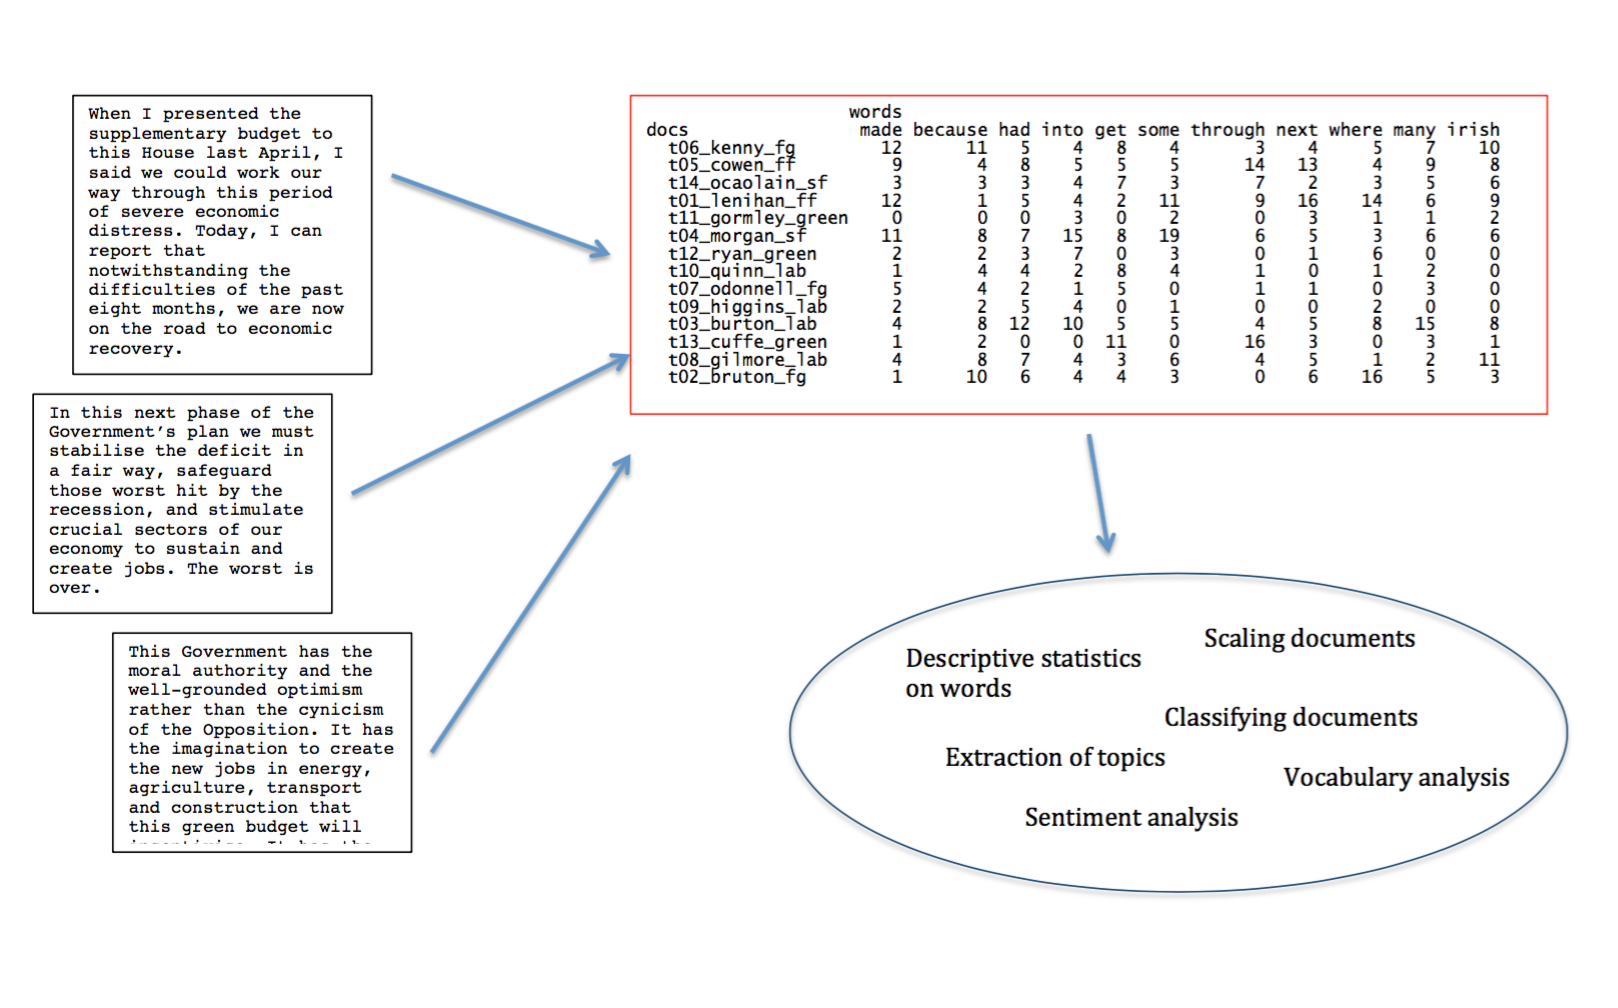
\includegraphics[scale=.4]{figures/qta-steps}
\end{center}
%\caption{\small{EU Enlargement in 2004}}
\end{figure}

\end{frame}
%%%%%%%%%%%%%%%%%%%%%%%%%%%%%%%%%%%%%%%%%%%%%%%%%%%%%%%%%%%%%%%%%%%%%%%%%





%%%%%%%%%%%%%%%%%%%%%%%%%%%%%%%%%%%%%%%%%%%%%%%%%%%%%%%%%%
\begin{frame}[fragile]{Step 1: Corpus Definition}

\begin{figure}[h]
\begin{center}
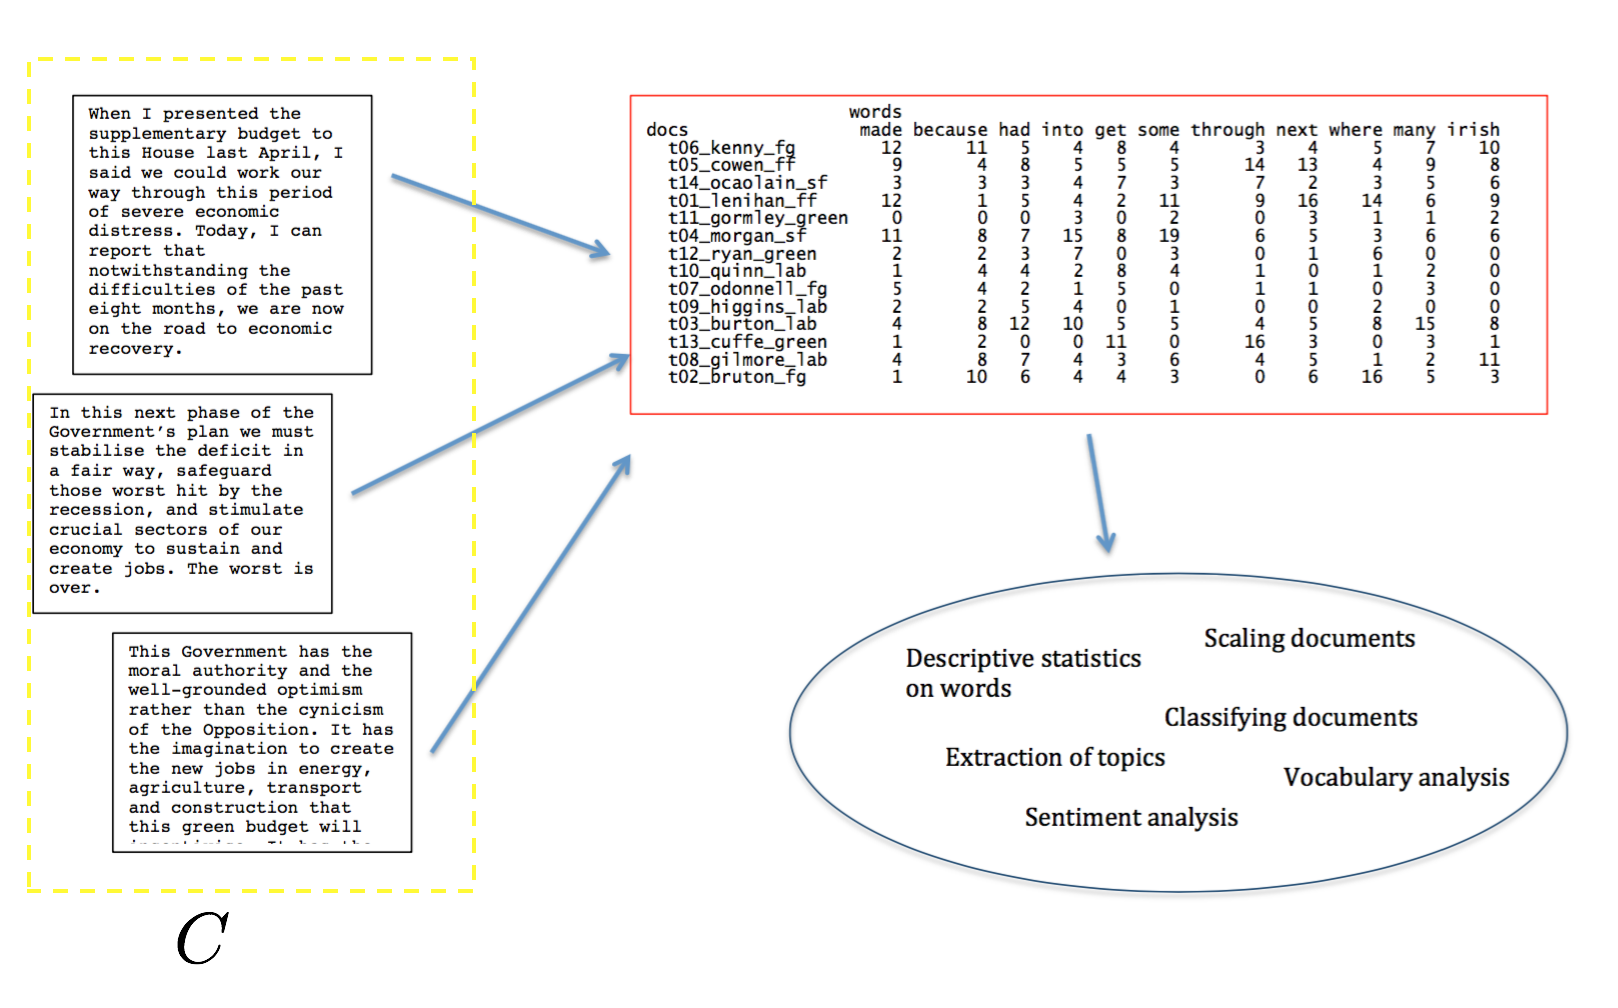
\includegraphics[scale=.2]{figures/qta-steps-corpus.png}
\end{center}
%\caption{\small{EU Enlargement in 2004}}
\end{figure}
First step consists of definition of \emph{corpus}
\begin{enumerate}

\item Selecting texts: definition of corpus of texts and being aware of underlying selection criteria.

\item Conversion of texts into a common electronic format

\item Defining documents: what will be the unit of analysis
\begin{itemize}
\item Sentence, Paragraph, Section, Chapter,...
\end{itemize}

\end{enumerate}

\end{frame}
%%%%%%%%%%%%%%%%%%%%%%%%%%%%%%%%%%%%%%%%%%%%%%%%%%%%%%%%%%%%%%%%%%%%%%%%%


%%%%%%%%%%%%%%%%%%%%%%%%%%%%%%%%%%%%%%%%%%%%%%%%%%%%%%%%%%
\begin{frame}[fragile]{Step 2: Feature Definition and Selection}

\begin{figure}[h]
\begin{center}
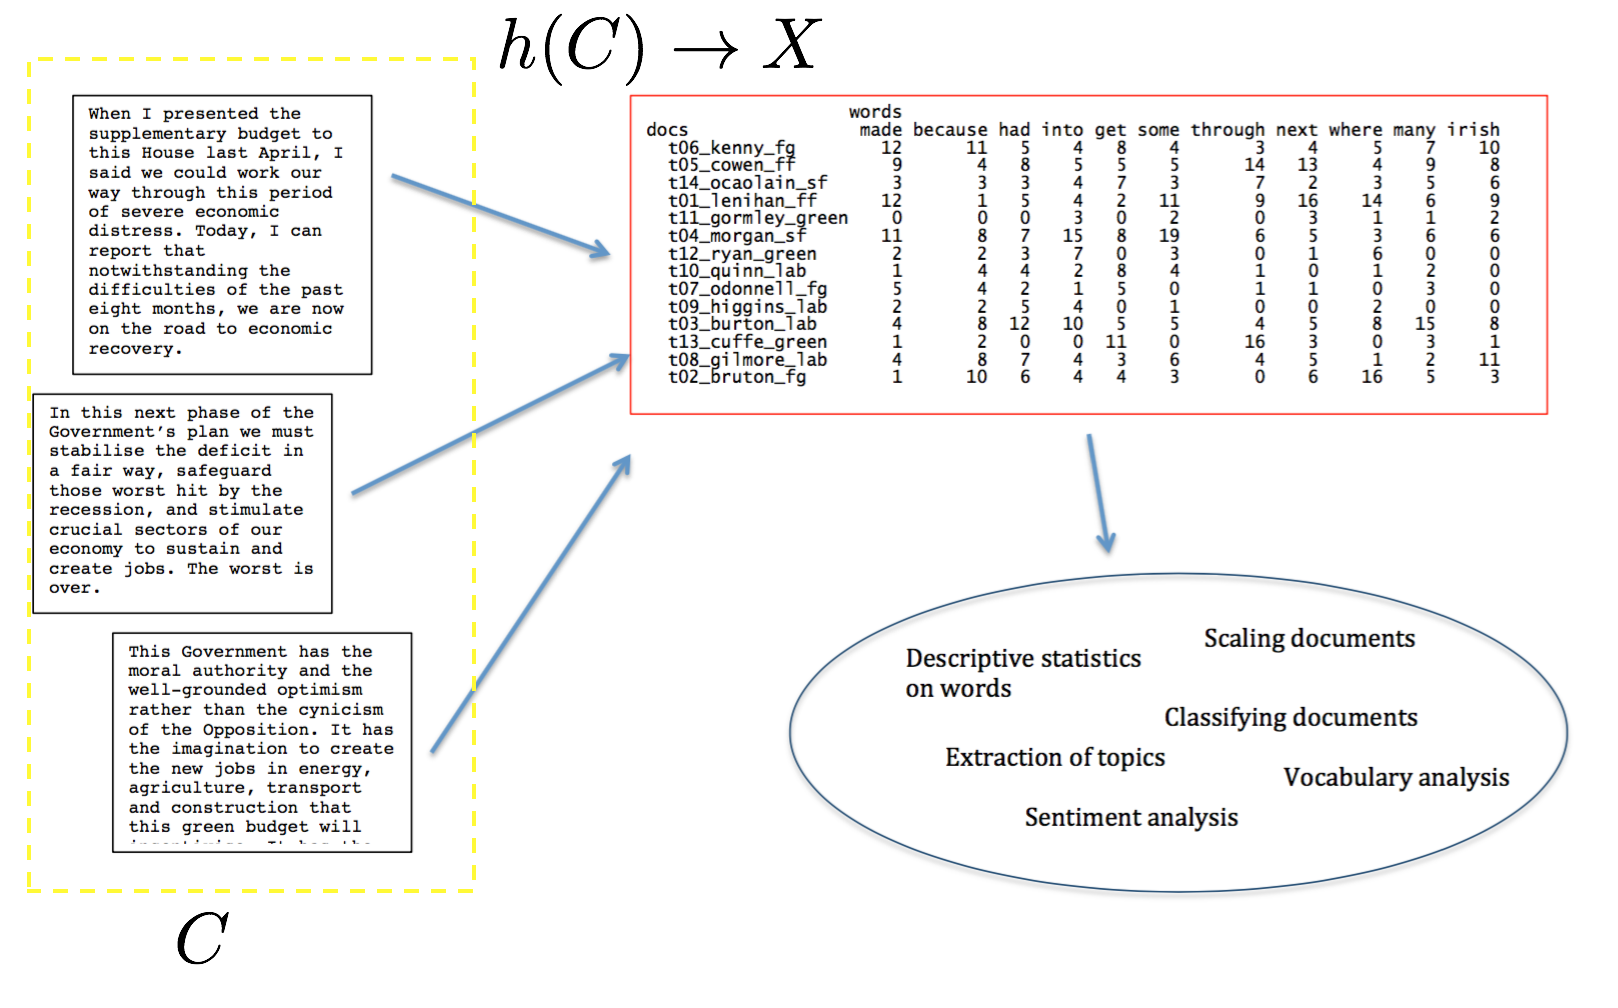
\includegraphics[scale=.2]{figures/qta-steps-corpus-h}
\end{center}
%\caption{\small{EU Enlargement in 2004}}
\end{figure}
Second step typically consists of definition of features 
\begin{enumerate}

\item This can be word tokens, \emph{n-grams}, keywords, indicators, patterns: challenge is to identify \emph{meaningful} features

\item For example: classification tasks you want to identify words that are characteristic and informative about underlying classes.

\item \emph{Curse of dimensionality}: Feature selection often required/desirable.

\item Convert corpus-features into a numerically accessible data matrix $X$
\end{enumerate}

\end{frame}
%%%%%%%%%%%%%%%%%%%%%%%%%%%%%%%%%%%%%%%%%%%%%%%%%%%%%%%%%%%%%%%%%%%%%%%%%




%%%%%%%%%%%%%%%%%%%%%%%%%%%%%%%%%%%%%%%%%%%%%%%%%%%%%%%%%%
\begin{frame}[fragile]{Step 3: Vector space representation \& analysis }

\begin{figure}[h]
\begin{center}
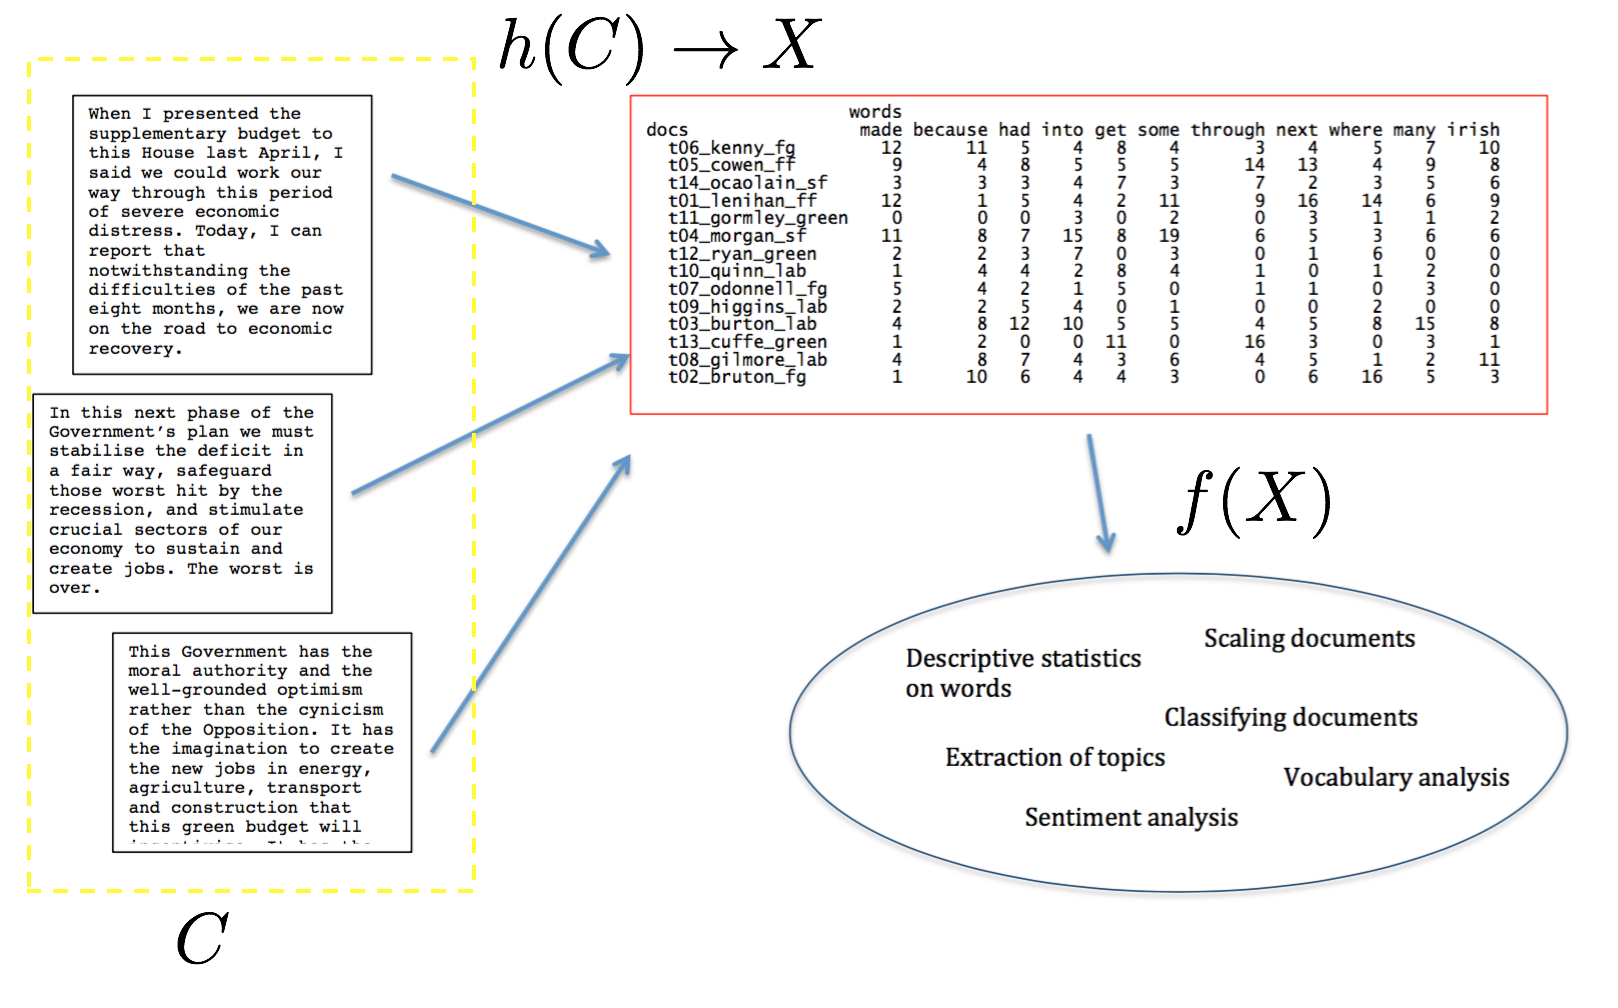
\includegraphics[scale=.2]{figures/qta-steps-corpus-f}
\end{center}
%\caption{\small{EU Enlargement in 2004}}
\end{figure}
Third step involves analyzing data repesentation to achieve a give task.
\begin{enumerate}

\item Classification (=Prediction): estimating a function $\hat{f}$ that maps individual documents $x_i$ into specific classes (e.g. republican versus democrat, sentiment label,...)

\item Clustering: identify groups of documents $x_i$ that are similar because they belong to similar latent class $C$, without knowing the set of classes \emph{ex ante}.

\end{enumerate}

\end{frame}
%%%%%%%%%%%%%%%%%%%%%%%%%%%%%%%%%%%%%%%%%%%%%%%%%%%%%%%%%%%%%%%%%%%%%%%%%




%%%%%%%%%%%%%%%%%%%%%%%%%%%%%%%%%%%%%%%%%%%%%%%%%%%%%%%%%%
\begin{frame}[fragile]{Some Terminology}

\begin{Description}
  \item[(text) corpus] usually a large set of documents that have limited structure. 
  \item[tokens] any word – so token count is total words
  \item[stems] word stems with suffixes removed 
  \item[lemmas] cannonical word forms: the base form of a word that has the same meaning even when different suffixes (or prefixes) are attached.
  \item[''key'' words]{words selected because of special attributes, meanings, or rates of occurrence}
  \item[stopwords] words that are excluded from text analysis for a range of reasons (typically lack of informational content)
  \item[complexity] word complexity usually measures the number of syllables
  \item[diversity] (lexical diversity) A measure of how many words occur per fixed word rate (a normalized vocabulary measure)
\end{Description}


\end{frame}
%%%%%%%%%%%%%%%%%%%%%%%%%%%%%%%%%%%%%%%%%%%%%%%%%%%%%%%%%%%%%%%%%%%%%%%%%

\section{Examples from Research}

%%%%%%%%%%%%%%%%%%%%%%%%%%%%%%%%%%%%%%%%%%%%%%%%%%%%%%%%%%
\begin{frame}[fragile]{Measuring Political Slant}
\begin{Description}
  \item[Reseach Question] Are newspapers maximizing profits by pandering to the ideology of their readership?
  \item[Corpus] Republican and democratic speeches, newspaper front page content
  \item[Features] Distincively Republican and Democratic n-grams
  \item[Analysis] \emph{Slant measure} of front page newspaper coverage picking up democratic vs. republican features. 
\end{Description}

See: Gentzkow, M., \& Shapiro, J. M. (2010). What Drives Media Slant? Evidence From U.S. Daily Newspapers. Econometrica, 78(1), 35–71.  

\end{frame}
%%%%%%%%%%%%%%%%%%%%%%%%%%%%%%%%%%%%%%%%%%%%%%%%%%%%%%%%%%%%%%%%%%%%%%%%%



%%%%%%%%%%%%%%%%%%%%%%%%%%%%%%%%%%%%%%%%%%%%%%%%%%%%%%%%%%
\begin{frame}[fragile]{Measuring Political Slant}
\begin{figure}[h]
\begin{center}
\includegraphics[scale=.5]<1>{figures/genzkow-democrat.png}
\includegraphics[scale=.5]<2>{figures/genzkow-republican.png}
\includegraphics[scale=.4]<3>{figures/slant-index.png}
\end{center}
%\caption{\small{EU Enlargement in 2004}}
\end{figure}

Identify n-grams (\emph{collocations}) and extract those that are distinctively more likely to appear in the corpus of republican versus democratic speaches congressional speeches
\end{frame}
%%%%%%%%%%%%%%%%%%%%%%%%%%%%%%%%%%%%%%%%%%%%%%%%%%%%%%%%%%%%%%%%%%%%%%%%%


%%%%%%%%%%%%%%%%%%%%%%%%%%%%%%%%%%%%%%%%%%%%%%%%%%%%%%%%%%
\begin{frame}[fragile]{Predicting National Identity}
\begin{Description}
  \item[Reseach Question] What are the costs of social ostracism? Evidence from two World Wars
  \item[Corpus] Names in census records
  \item[Features] Distinctly german letter combinations, suffixes in names and surnames
  \item[Analysis] Predict national identity and study evolution of distinctively German (+Asian) names.   
\end{Description}

Use machine learning model to predict national identity and study evolution over time. Are there non-linearities in underlying assimmilation pressures? What is the case if (national) identity is non-malleable. This is ongoing research.
\end{frame}
%%%%%%%%%%%%%%%%%%%%%%%%%%%%%%%%%%%%%%%%%%%%%%%%%%%%%%%%%%%%%%%%%%%%%%%%%



%%%%%%%%%%%%%%%%%%%%%%%%%%%%%%%%%%%%%%%%%%%%%%%%%%%%%%%%%%
\begin{frame}[fragile]{Predicting National Identity}
\begin{figure}[h]
\begin{center}
\includegraphics[scale=.3]<1>{figures/anti-german}
\includegraphics[scale=.3]<2>{figures/letter-combinations-features}
\includegraphics[scale=.3]<2>{figures/letter-comb-features2}
\end{center}
%\caption{\small{EU Enlargement in 2004}}
\end{figure}

Build a predictive model based on common names identified using a Lasso and include dummy coded features extracted using \emph{regular expressions}. 
\end{frame}
%%%%%%%%%%%%%%%%%%%%%%%%%%%%%%%%%%%%%%%%%%%%%%%%%%%%%%%%%%%%%%%%%%%%%%%%%



%%%%%%%%%%%%%%%%%%%%%%%%%%%%%%%%%%%%%%%%%%%%%%%%%%%%%%%%%%
\begin{frame}[fragile]{Measuring Policy Uncertainty}
\begin{Description}
  \item[Reseach Question] Construct a measure of policy uncertainty (second moment shocks) to study economic effects.
  \item[Corpus] Digital archives of newspaper
  \item[Features] Counting articles (``uncertain'' OR ``uncertainty'')  AND (``economic'' OR ``economy'') AND (``congress'' OR ``deficit'' OR ``federal reserve'' OR ``legislation'' OR ``regulation'' OR ``white house'') normalize article counts by total newspaper articles that month.
  \item[Analysis] Perform econometric analysis on resulting index.
\end{Description}

Baker, Bloom, and Davis measure economic policy uncertainty using Boolean search of newspaper articles: \url{http://www.policyuncertainty.com/}.
\end{frame}
%%%%%%%%%%%%%%%%%%%%%%%%%%%%%%%%%%%%%%%%%%%%%%%%%%%%%%%%%%%%%%%%%%%%%%%%%


%%%%%%%%%%%%%%%%%%%%%%%%%%%%%%%%%%%%%%%%%%%%%%%%%%%%%%%%%%
\begin{frame}[fragile]{Measuring Policy Uncertainty}
\begin{figure}[h]
\begin{center}
\includegraphics[scale=.5]<1>{figures/policy-uncertainty}
\end{center}
%\caption{\small{EU Enlargement in 2004}}
\end{figure}

Baker, Bloom, and Davis measure economic policy uncertainty using Boolean search of newspaper articles: \url{http://www.policyuncertainty.com/}.
\end{frame}
%%%%%%%%%%%%%%%%%%%%%%%%%%%%%%%%%%%%%%%%%%%%%%%%%%%%%%%%%%%%%%%%%%%%%%%%%




%%%%%%%%%%%%%%%%%%%%%%%%%%%%%%%%%%%%%%%%%%%%%%%%%%%%%%%%%%
\begin{frame}[fragile]{Measuring Consumer Confidence}
\begin{Description}
  \item[Reseach Question] Can Twitter feeds be used to construct consumer high frequency consumer confidence time series?
  \item[Corpus] A large collection of twitter feeds
  \item[Features] Fragments of text around topic keywords: \emph{economy}, \emph{job}.
  \item[Analysis] (Heuristic) Approach measuring ratio of positive versus negative coded words around topic keywords. 
\end{Description}

O'Connor, B., Balasubramanyan, R., Routledge, B. R., \& Smith, N. a. (2010). From tweets to polls: Linking text sentiment to public opinion time series. 
\end{frame}
%%%%%%%%%%%%%%%%%%%%%%%%%%%%%%%%%%%%%%%%%%%%%%%%%%%%%%%%%%%%%%%%%%%%%%%%%


%%%%%%%%%%%%%%%%%%%%%%%%%%%%%%%%%%%%%%%%%%%%%%%%%%%%%%%%%%
\begin{frame}[fragile]{Measuring Consumer Confidence}
\begin{figure}[h]
\begin{center}
\includegraphics[scale=.45]<1>{figures/twitter-sentiment.png}
\end{center}
%\caption{\small{EU Enlargement in 2004}}
\end{figure}

O'Connor, B., Balasubramanyan, R., Routledge, B. R., \& Smith, N. a. (2010). From tweets to polls: Linking text sentiment to public opinion time series. 
\end{frame}
%%%%%%%%%%%%%%%%%%%%%%%%%%%%%%%%%%%%%%%%%%%%%%%%%%%%%%%%%%%%%%%%%%%%%%%%%


%%%%%%%%%%%%%%%%%%%%%%%%%%%%%%%%%%%%%%%%%%%%%%%%%%%%%%%%%%
\begin{frame}[fragile]{Retrieving (Conflict) Event Information}
\begin{Description}
  \item[Reseach Question] Automatically extract (conflict) event information from textual data. 
  \item[Corpus] Digital archive of newspaper clippings about conflict in South Asia.
  \item[Features] Individual sentences in newspaper article.
  \item[Analysis] Extract linguistic features to fill event tuple: Subject, Verb, Object pairs and certain Named Entities (Location, Date)
\end{Description}

Fetzer, T. (2016) Social Insurance and Conflict: Evidence from India, mimeo.
\end{frame}
%%%%%%%%%%%%%%%%%%%%%%%%%%%%%%%%%%%%%%%%%%%%%%%%%%%%%%%%%%%%%%%%%%%%%%%%%


%%%%%%%%%%%%%%%%%%%%%%%%%%%%%%%%%%%%%%%%%%%%%%%%%%%%%%%%%%
\begin{frame}[fragile]{Retrieving (Conflict) Event Information}
\begin{figure}[h]
\begin{center}
\includegraphics[scale=.6]<1>{figures/sentence-fragments.png}
\includegraphics[scale=.7]<2>{figures/event-tuple.png}
\end{center}
%\caption{\small{EU Enlargement in 2004}}
\end{figure}

Fetzer, T. (2016) Social Insurance and Conflict: Evidence from India, mimeo.
\end{frame}
%%%%%%%%%%%%%%%%%%%%%%%%%%%%%%%%%%%%%%%%%%%%%%%%%%%%%%%%%%%%%%%%%%%%%%%%%



\section{An Introduction to R}


%%%%%%%%%%%%%%%%%%%%%%%%%%%%%%%%%%%%%%%%%%%%%%%%%%%%%%%%%%
\begin{frame}[fragile]{Learning \code{R} is an investment}

\begin{center}
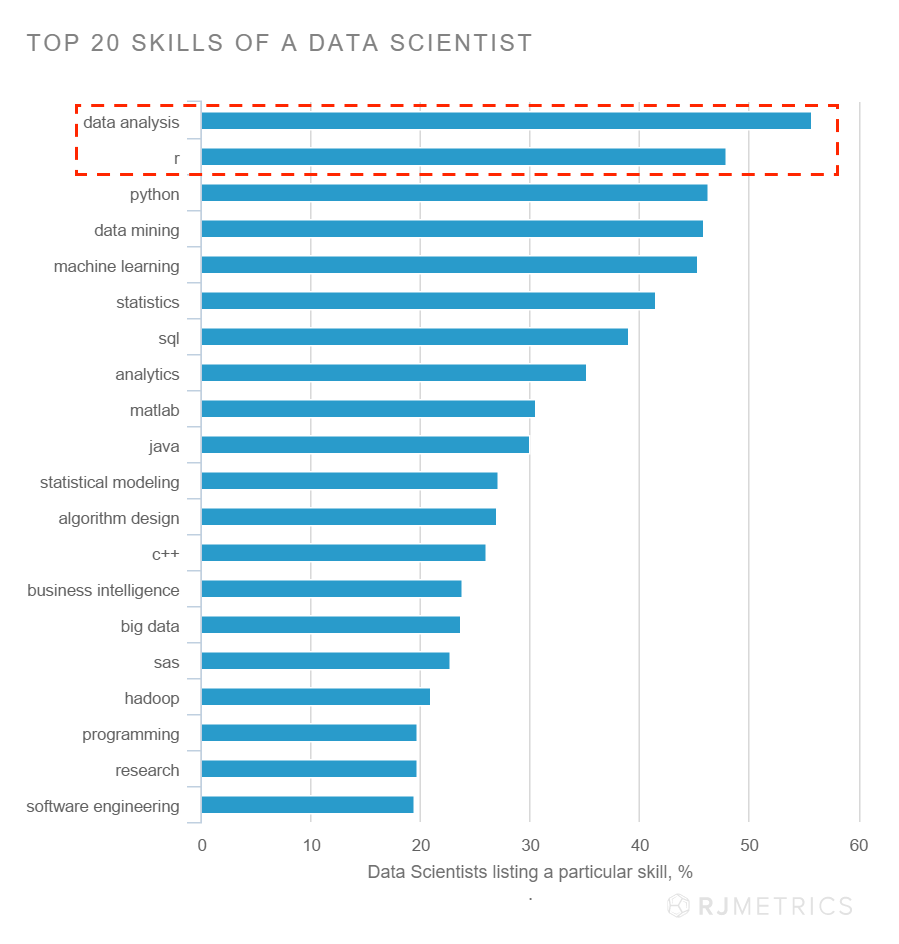
\includegraphics[scale=0.35]{figures/learning-R.png}
\end{center}


\end{frame}
%%%%%%%%%%%%%%%%%%%%%%%%%%%%%%%%%%%%%%%%%%%%%%%%%%%%%%%%%%%%%%%%%%%%%%%%%


%%%%%%%%%%%%%%%%%%%%%%%%%%%%%%%%%%%%%%%%%%%%%%%%%%%%%%%%%%
\begin{frame}[fragile]{Advantages of \code{R}}

\begin{itemize}

\item Many of you will have some form of prior experience with various programming languages.\smallskip

\item Separation of tasks is quite common: Python often used for \emph{web scraping}, \emph{Stata} used by some for data cleaning and analysis, \emph{ArcGIS} or \emph{QGIS} (and indirectly python) for spatial analysis,... \smallskip

\item Beautiful feature of $R$ is its versatility due to the many extensions.



\end{itemize}



\end{frame}
%%%%%%%%%%%%%%%%%%%%%%%%%%%%%%%%%%%%%%%%%%%%%%%%%%%%%%%%%%%%%%%%%%%%%%%%%



%%%%%%%%%%%%%%%%%%%%%%%%%%%%%%%%%%%%%%%%%%%%%%%%%%%%%%%%%%
\begin{frame}[fragile]{Getting started with \code{R}: Rstudio}
\begin{quote} RStudio is a free and open-source integrated development environment (IDE) for R, a programming language for statistical computing and graphics.\end{quote}

\begin{center}
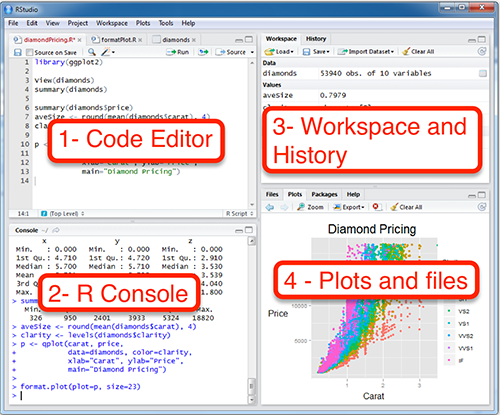
\includegraphics[scale=0.6]{figures/rstudio.png}
\end{center}
\url{https://www.rstudio.com/products/rstudio/download/}
Alternatively: work in Terminal (command line) or using the R-gui that is shipped with base-R.
\end{frame}
%%%%%%%%%%%%%%%%%%%%%%%%%%%%%%%%%%%%%%%%%%%%%%%%%%%%%%%%%%%%%%%%%%%%%%%%%



%%%%%%%%%%%%%%%%%%%%%%%%%%%%%%%%%%%%%%%%%%%%%%%%%%%%%%%%%%
\begin{frame}[fragile]{Markdown for homeworks}

R Markdown makes it easy to turn analyses in R into simple documents or reports. 
\begin{center}

\includegraphics[scale=0.2]<1>{figures/rmarkdown-example.png}
\includegraphics[scale=0.2]<2>{figures/rmarkdown-example.png}

\end{center}

You will be asked to provide homeworks in R-Markdown format. You will You can describe in the Markdown document what, why and how you proceed with your analysis proiding the code an the results in a simple document.

\end{frame}
%%%%%%%%%%%%%%%%%%%%%%%%%%%%%%%%%%%%%%%%%%%%%%%%%%%%%%%%%%%%%%%%%%%%%%%%%



%%%%%%%%%%%%%%%%%%%%%%%%%%%%%%%%%%%%%%%%%%%%%%%%%%%%%%%%%%
\begin{frame}[fragile]{Data Types}


These are the basic data types
\begin{Description}

\item[numeric] 8-byte numeric representations\smallskip

\item[integer] non-floating point numbers\smallskip

\item[character] text\smallskip

\item[logical] \code{TRUE} or \code{FALSE}\smallskip

\end{Description}

Recursive types also exist, such as lists and vectors; there are also special classifications for \code{NA}.

\end{frame}
%%%%%%%%%%%%%%%%%%%%%%%%%%%%%%%%%%%%%%%%%%%%%%%%%%%%%%%%%%%%%%%%%%%%%%%%%





%%%%%%%%%%%%%%%%%%%%%%%%%%%%%%%%%%%%%%%%%%%%%%%%%%%%%%%%%%
\begin{frame}[fragile]{Data Types: Integer}
\begin{knitrout}\tiny
\definecolor{shadecolor}{rgb}{0.969, 0.969, 0.969}\color{fgcolor}\begin{kframe}
\begin{alltt}
\hlstd{x} \hlkwb{<-} \hlnum{10}
\hlkwd{typeof}\hlstd{(x)}
\end{alltt}
\begin{verbatim}
## [1] "double"
\end{verbatim}
\begin{alltt}
\hlkwd{is.integer}\hlstd{(x)}
\end{alltt}
\begin{verbatim}
## [1] FALSE
\end{verbatim}
\begin{alltt}
\hlstd{x} \hlkwb{<-} \hlnum{7L}
\hlkwd{typeof}\hlstd{(x)}
\end{alltt}
\begin{verbatim}
## [1] "integer"
\end{verbatim}
\begin{alltt}
\hlkwd{object.size}\hlstd{(x)}
\end{alltt}
\begin{verbatim}
## 48 bytes
\end{verbatim}
\begin{alltt}
\hlkwd{as.integer}\hlstd{(}\hlnum{3.14}\hlstd{)}
\end{alltt}
\begin{verbatim}
## [1] 3
\end{verbatim}
\end{kframe}
\end{knitrout}


\end{frame}
%%%%%%%%%%%%%%%%%%%%%%%%%%%%%%%%%%%%%%%%%%%%%%%%%%%%%%%%%%%%%%%%%%%%%%%%%


%%%%%%%%%%%%%%%%%%%%%%%%%%%%%%%%%%%%%%%%%%%%%%%%%%%%%%%%%%
\begin{frame}[fragile]{Data Types: Character}
\begin{knitrout}\tiny
\definecolor{shadecolor}{rgb}{0.969, 0.969, 0.969}\color{fgcolor}\begin{kframe}
\begin{alltt}
\hlkwd{typeof}\hlstd{(}\hlstr{"test string"}\hlstd{)}
\end{alltt}
\begin{verbatim}
## [1] "character"
\end{verbatim}
\begin{alltt}
\hlkwd{object.size}\hlstd{(}\hlstr{"a"}\hlstd{)}
\end{alltt}
\begin{verbatim}
## 96 bytes
\end{verbatim}
\begin{alltt}
\hlstd{s} \hlkwb{<-} \hlstr{""} \hlcom{# Unicode cat(s)}

\hlkwd{as.character}\hlstd{(}\hlstr{"3.14"}\hlstd{)} \hlcom{# coerce numerics to character }
\end{alltt}
\begin{verbatim}
## [1] "3.14"
\end{verbatim}
\end{kframe}
\end{knitrout}
\end{frame}
%%%%%%%%%%%%%%%%%%%%%%%%%%%%%%%%%%%%%%%%%%%%%%%%%%%%%%%%%%%%%%%%%%%%%%%%%


%%%%%%%%%%%%%%%%%%%%%%%%%%%%%%%%%%%%%%%%%%%%%%%%%%%%%%%%%%
\begin{frame}[fragile]{Data Types: numeric}
\begin{knitrout}\tiny
\definecolor{shadecolor}{rgb}{0.969, 0.969, 0.969}\color{fgcolor}\begin{kframe}
\begin{alltt}
\hlstd{x} \hlkwb{<-} \hlnum{10.5}

\hlkwd{typeof}\hlstd{(x)}
\end{alltt}
\begin{verbatim}
## [1] "double"
\end{verbatim}
\begin{alltt}
\hlkwd{object.size}\hlstd{(x)}
\end{alltt}
\begin{verbatim}
## 48 bytes
\end{verbatim}
\end{kframe}
\end{knitrout}

\end{frame}
%%%%%%%%%%%%%%%%%%%%%%%%%%%%%%%%%%%%%%%%%%%%%%%%%%%%%%%%%%%%%%%%%%%%%%%%%


%%%%%%%%%%%%%%%%%%%%%%%%%%%%%%%%%%%%%%%%%%%%%%%%%%%%%%%%%%
\begin{frame}[fragile]{Data Types: factor}
\begin{knitrout}\tiny
\definecolor{shadecolor}{rgb}{0.969, 0.969, 0.969}\color{fgcolor}\begin{kframe}
\begin{alltt}
\hlcom{#create random sample of letters abcd drawn with replacement}
\hlstd{x}\hlkwb{<-}\hlkwd{sample}\hlstd{(letters[}\hlnum{1}\hlopt{:}\hlnum{4}\hlstd{],} \hlnum{50}\hlstd{,} \hlkwc{replace} \hlstd{=}\hlnum{TRUE}\hlstd{)}
\hlkwd{head}\hlstd{(x)}
\end{alltt}
\begin{verbatim}
## [1] "b" "c" "d" "b" "b" "b"
\end{verbatim}
\begin{alltt}
\hlstd{x}\hlkwb{<-}\hlkwd{factor}\hlstd{(x)}
\hlstd{x}
\end{alltt}
\begin{verbatim}
##  [1] b c d b b b c d d c a a d b a d a c b d b a c d c a a c a a d b c c d c d c d a b d d
## [44] d c b a c c c
## Levels: a b c d
\end{verbatim}
\begin{alltt}
\hlkwd{levels}\hlstd{(x)}
\end{alltt}
\begin{verbatim}
## [1] "a" "b" "c" "d"
\end{verbatim}
\end{kframe}
\end{knitrout}
Factors are more efficiently stored compared to strings as they are coded as numeric values. It can be dangerous. Setting:

\code{options(stringsAsFactors=FALSE)}

ensures that when creating data frames, strings are not automatically replaced as factors.

\end{frame}
%%%%%%%%%%%%%%%%%%%%%%%%%%%%%%%%%%%%%%%%%%%%%%%%%%%%%%%%%%%%%%%%%%%%%%%%%



%%%%%%%%%%%%%%%%%%%%%%%%%%%%%%%%%%%%%%%%%%%%%%%%%%%%%%%%%%
\begin{frame}[fragile]{Data Types: \code{is.*()} and \code{as.*()}}
\begin{knitrout}\tiny
\definecolor{shadecolor}{rgb}{0.969, 0.969, 0.969}\color{fgcolor}\begin{kframe}
\begin{alltt}
\hlkwd{is.numeric}\hlstd{(x)}
\end{alltt}
\begin{verbatim}
## [1] FALSE
\end{verbatim}
\begin{alltt}
\hlkwd{is.numeric}\hlstd{(}\hlnum{7.1}\hlstd{)}
\end{alltt}
\begin{verbatim}
## [1] TRUE
\end{verbatim}
\begin{alltt}
\hlkwd{is.numeric}\hlstd{(}\hlstr{"7.1"}\hlstd{)}
\end{alltt}
\begin{verbatim}
## [1] FALSE
\end{verbatim}
\begin{alltt}
\hlkwd{is.numeric}\hlstd{(}\hlkwd{as.numeric}\hlstd{(}\hlstr{"7.1"}\hlstd{))}
\end{alltt}
\begin{verbatim}
## [1] TRUE
\end{verbatim}
\end{kframe}
\end{knitrout}

\end{frame}
%%%%%%%%%%%%%%%%%%%%%%%%%%%%%%%%%%%%%%%%%%%%%%%%%%%%%%%%%%%%%%%%%%%%%%%%%


%%%%%%%%%%%%%%%%%%%%%%%%%%%%%%%%%%%%%%%%%%%%%%%%%%%%%%%%%%
\begin{frame}[fragile]{Data Structures}
R operates on named \emph{data structures}. The simplest such structure is a numeric vector, which is a single entity consisting of a collection of numbers. 
\begin{knitrout}\tiny
\definecolor{shadecolor}{rgb}{0.969, 0.969, 0.969}\color{fgcolor}\begin{kframe}
\begin{alltt}
\hlstd{x} \hlkwb{<-} \hlkwd{c}\hlstd{(}\hlnum{10.4}\hlstd{,} \hlnum{5.6}\hlstd{,} \hlnum{3.1}\hlstd{,} \hlnum{6.4}\hlstd{,} \hlnum{21.7}\hlstd{)}
\hlstd{x}
\end{alltt}
\begin{verbatim}
## [1] 10.4  5.6  3.1  6.4 21.7
\end{verbatim}
\begin{alltt}
\hlkwd{class}\hlstd{(x)}
\end{alltt}
\begin{verbatim}
## [1] "numeric"
\end{verbatim}
\begin{alltt}
\hlkwd{length}\hlstd{(x)}
\end{alltt}
\begin{verbatim}
## [1] 5
\end{verbatim}
\begin{alltt}
\hlstd{b}\hlkwb{<-}\hlkwd{c}\hlstd{(x,}\hlstr{"test"}\hlstd{)}
\hlkwd{class}\hlstd{(b)}
\end{alltt}
\begin{verbatim}
## [1] "character"
\end{verbatim}
\end{kframe}
\end{knitrout}
Operations on vectors are element by element.
\begin{knitrout}\tiny
\definecolor{shadecolor}{rgb}{0.969, 0.969, 0.969}\color{fgcolor}\begin{kframe}
\begin{alltt}
\hlstd{z} \hlkwb{<-} \hlkwd{sqrt}\hlstd{(x)}
\hlstd{z}\hlopt{*}\hlkwd{sqrt}\hlstd{(x)}
\end{alltt}
\begin{verbatim}
## [1] 10.4  5.6  3.1  6.4 21.7
\end{verbatim}
\begin{alltt}
\hlcom{#vector - dot product}
\hlstd{z} \hlopt \hlkwd{sqrt}\hlstd{(x)}
\end{alltt}
\begin{verbatim}
##      [,1]
## [1,] 47.2
\end{verbatim}
\end{kframe}
\end{knitrout}

\end{frame}
%%%%%%%%%%%%%%%%%%%%%%%%%%%%%%%%%%%%%%%%%%%%%%%%%%%%%%%%%%%%%%%%%%%%%%%%%


%%%%%%%%%%%%%%%%%%%%%%%%%%%%%%%%%%%%%%%%%%%%%%%%%%%%%%%%%%
\begin{frame}[fragile]{Selecting and modifying subsets of a data set}
You can select data or subset data using logical conditions in \code{[]}.
\begin{knitrout}\tiny
\definecolor{shadecolor}{rgb}{0.969, 0.969, 0.969}\color{fgcolor}\begin{kframe}
\begin{alltt}
\hlstd{x} \hlkwb{<-} \hlkwd{c}\hlstd{(x,} \hlnum{1}\hlopt{/}\hlnum{0}\hlstd{)}
\hlstd{x}
\end{alltt}
\begin{verbatim}
## [1] 10.4  5.6  3.1  6.4 21.7  Inf
\end{verbatim}
\begin{alltt}
\hlstd{x[}\hlkwd{is.infinite}\hlstd{(x)]}
\end{alltt}
\begin{verbatim}
## [1] Inf
\end{verbatim}
\begin{alltt}
\hlkwd{is.infinite}\hlstd{(x)}
\end{alltt}
\begin{verbatim}
## [1] FALSE FALSE FALSE FALSE FALSE  TRUE
\end{verbatim}
\begin{alltt}
\hlstd{x[}\hlkwd{which.max}\hlstd{(x)]}
\end{alltt}
\begin{verbatim}
## [1] Inf
\end{verbatim}
\begin{alltt}
\hlstd{x[}\hlopt{!}\hlkwd{is.infinite}\hlstd{(x)]}
\end{alltt}
\begin{verbatim}
## [1] 10.4  5.6  3.1  6.4 21.7
\end{verbatim}
\begin{alltt}
\hlstd{x[}\hlnum{1}\hlopt{:}\hlnum{4}\hlstd{]}
\end{alltt}
\begin{verbatim}
## [1] 10.4  5.6  3.1  6.4
\end{verbatim}
\begin{alltt}
\hlstd{x[}\hlopt{-}\hlnum{6}\hlstd{]}
\end{alltt}
\begin{verbatim}
## [1] 10.4  5.6  3.1  6.4 21.7
\end{verbatim}
\end{kframe}
\end{knitrout}
\end{frame}
%%%%%%%%%%%%%%%%%%%%%%%%%%%%%%%%%%%%%%%%%%%%%%%%%%%%%%%%%%%%%%%%%%%%%%%%%



%%%%%%%%%%%%%%%%%%%%%%%%%%%%%%%%%%%%%%%%%%%%%%%%%%%%%%%%%%
\begin{frame}[fragile]{Functions}
\begin{knitrout}\tiny
\definecolor{shadecolor}{rgb}{0.969, 0.969, 0.969}\color{fgcolor}\begin{kframe}
\begin{alltt}
\hlstd{plusOne} \hlkwb{<-} \hlkwa{function}\hlstd{(}\hlkwc{x}\hlstd{)\{}
        \hlkwd{return}\hlstd{(x}\hlopt{+}\hlnum{1}\hlstd{)}
        \hlstd{\}}

\hlstd{plusOne2} \hlkwb{<-} \hlkwa{function}\hlstd{(}\hlkwc{num}\hlstd{)\{}
                \hlkwd{return}\hlstd{(num}\hlopt{+}\hlnum{1}\hlstd{)}
        \hlstd{\}}

        \hlkwd{plusOne}\hlstd{(}\hlnum{8}\hlstd{)}
\end{alltt}
\begin{verbatim}
## [1] 9
\end{verbatim}
\begin{alltt}
        \hlkwd{plusOne2}\hlstd{(}\hlnum{10}\hlstd{)}
\end{alltt}
\begin{verbatim}
## [1] 11
\end{verbatim}
\begin{alltt}
  \hlkwd{plusOne2}\hlstd{(}\hlkwc{num}\hlstd{=}\hlnum{5}\hlstd{)}
\end{alltt}
\begin{verbatim}
## [1] 6
\end{verbatim}
\begin{alltt}
  \hlcom{#plusOne2(wrongVar=2)}
\end{alltt}
\end{kframe}
\end{knitrout}
\end{frame}
%%%%%%%%%%%%%%%%%%%%%%%%%%%%%%%%%%%%%%%%%%%%%%%%%%%%%%%%%%%%%%%%%%%%%%%%%


%%%%%%%%%%%%%%%%%%%%%%%%%%%%%%%%%%%%%%%%%%%%%%%%%%%%%%%%%%
\begin{frame}[fragile]{Loops}
\begin{knitrout}\tiny
\definecolor{shadecolor}{rgb}{0.969, 0.969, 0.969}\color{fgcolor}\begin{kframe}
\begin{alltt}
  \hlkwa{for} \hlstd{(number} \hlkwa{in} \hlnum{1}\hlopt{:}\hlnum{5}\hlstd{)\{}
        \hlkwd{print} \hlstd{(number)}
\hlstd{\}}
\end{alltt}
\begin{verbatim}
## [1] 1
## [1] 2
## [1] 3
## [1] 4
## [1] 5
\end{verbatim}
\begin{alltt}
\hlcom{#Looping over functions}
\hlstd{a} \hlkwb{<-} \hlkwd{c}\hlstd{(}\hlnum{1}\hlstd{,}\hlnum{2}\hlstd{,}\hlnum{3}\hlstd{,}\hlnum{4}\hlstd{,}\hlnum{5}\hlstd{)}
\hlkwa{for} \hlstd{(value} \hlkwa{in} \hlstd{a)\{}
        \hlkwd{print} \hlstd{(}
                \hlkwd{plusOne}\hlstd{(value)}
        \hlstd{)}
\hlstd{\}}
\end{alltt}
\begin{verbatim}
## [1] 2
## [1] 3
## [1] 4
## [1] 5
## [1] 6
\end{verbatim}
\begin{alltt}
\hlstd{listOfNumbers} \hlkwb{<-} \hlkwd{c}\hlstd{(}\hlnum{1}\hlstd{,}\hlnum{2}\hlstd{,}\hlnum{3}\hlstd{,}\hlnum{4}\hlstd{,}\hlnum{5}\hlstd{)}
\hlkwa{for} \hlstd{(number} \hlkwa{in} \hlstd{listOfNumbers)\{}
        \hlkwd{print} \hlstd{(}
                \hlstd{number}\hlopt{+}\hlnum{1}
        \hlstd{)}
\hlstd{\}}
\end{alltt}
\begin{verbatim}
## [1] 2
## [1] 3
## [1] 4
## [1] 5
## [1] 6
\end{verbatim}
\begin{alltt}
\hlstd{a} \hlkwb{<-} \hlkwd{c}\hlstd{(}\hlnum{1}\hlstd{,}\hlnum{2}\hlstd{,}\hlnum{3}\hlstd{,}\hlnum{4}\hlstd{,}\hlnum{5}\hlstd{)}

\hlkwa{for} \hlstd{(i} \hlkwa{in} \hlnum{1}\hlopt{:}\hlkwd{length}\hlstd{(a))\{}
        \hlkwd{print} \hlstd{(}
                \hlkwd{plusOne}\hlstd{(a[i])}
        \hlstd{)}
\hlstd{\}}
\end{alltt}
\begin{verbatim}
## [1] 2
## [1] 3
## [1] 4
## [1] 5
## [1] 6
\end{verbatim}
\end{kframe}
\end{knitrout}
\end{frame}
%%%%%%%%%%%%%%%%%%%%%%%%%%%%%%%%%%%%%%%%%%%%%%%%%%%%%%%%%%%%%%%%%%%%%%%%%


%%%%%%%%%%%%%%%%%%%%%%%%%%%%%%%%%%%%%%%%%%%%%%%%%%%%%%%%%%
\begin{frame}[fragile]{Complex Data Structures: Matrices}
Matrices combine data vectors coercing a common type: all vectors that make up a matrix have same data type (e.g. numeric, character).
\begin{knitrout}\tiny
\definecolor{shadecolor}{rgb}{0.969, 0.969, 0.969}\color{fgcolor}\begin{kframe}
\begin{alltt}
\hlstd{x}\hlkwb{<-}\hlkwd{rnorm}\hlstd{(}\hlkwc{n}\hlstd{=}\hlnum{26}\hlstd{)}
\hlstd{y}\hlkwb{<-}\hlkwd{runif}\hlstd{(}\hlkwc{n}\hlstd{=}\hlnum{26}\hlstd{)}
\hlstd{MAT}\hlkwb{<-}\hlkwd{cbind}\hlstd{(x,y)}
\hlkwd{class}\hlstd{(MAT)}
\end{alltt}
\begin{verbatim}
## [1] "matrix"
\end{verbatim}
\begin{alltt}
\hlkwd{rownames}\hlstd{(MAT)} \hlkwb{<-} \hlnum{1}\hlopt{:}\hlkwd{nrow}\hlstd{(MAT)}
\hlkwd{colnames}\hlstd{(MAT)} \hlkwb{<-} \hlkwd{c}\hlstd{(}\hlstr{"x"}\hlstd{,}\hlstr{"y"}\hlstd{)}

\hlcom{#subsetting}
\hlstd{MAT[}\hlnum{12}\hlstd{,}\hlstr{"y"}\hlstd{]}
\end{alltt}
\begin{verbatim}
## [1] 0.0373
\end{verbatim}
\begin{alltt}
\hlstd{MAT[}\hlnum{12}\hlstd{,]}
\end{alltt}
\begin{verbatim}
##       x       y 
## -1.9274  0.0373
\end{verbatim}
\begin{alltt}
\hlkwd{head}\hlstd{(letters)}
\end{alltt}
\begin{verbatim}
## [1] "a" "b" "c" "d" "e" "f"
\end{verbatim}
\begin{alltt}
\hlstd{MAT}\hlkwb{<-}\hlkwd{cbind}\hlstd{(MAT, letters)}
\hlcom{#adding a character column changes type of all elements}
\hlkwd{head}\hlstd{(MAT)}
\end{alltt}
\begin{verbatim}
##   x                     y                   letters
## 1 "2.13631660354939"    "0.364831202430651" "a"    
## 2 "1.21815435633569"    "0.222715873736888" "b"    
## 3 "-1.62450225224365"   "0.298199398675933" "c"    
## 4 "-0.0354296365102945" "0.796236804686487" "d"    
## 5 "-1.9211767346097"    "0.688834731001407" "e"    
## 6 "0.754742543238073"   "0.903118321672082" "f"
\end{verbatim}
\end{kframe}
\end{knitrout}
\end{frame}
%%%%%%%%%%%%%%%%%%%%%%%%%%%%%%%%%%%%%%%%%%%%%%%%%%%%%%%%%%%%%%%%%%%%%%%%%


%%%%%%%%%%%%%%%%%%%%%%%%%%%%%%%%%%%%%%%%%%%%%%%%%%%%%%%%%%
\begin{frame}[fragile]{Complex Data Structures: data.frame}
data.frames allow the combination of multiple object types without their underlying types being changed. This is the central data object that is typically worked with.
\begin{knitrout}\tiny
\definecolor{shadecolor}{rgb}{0.969, 0.969, 0.969}\color{fgcolor}\begin{kframe}
\begin{alltt}
\hlstd{x}\hlkwb{<-}\hlkwd{rnorm}\hlstd{(}\hlkwc{n}\hlstd{=}\hlnum{26}\hlstd{)}
\hlstd{y}\hlkwb{<-}\hlkwd{runif}\hlstd{(}\hlkwc{n}\hlstd{=}\hlnum{26}\hlstd{)}
\hlstd{DF}\hlkwb{<-}\hlkwd{data.frame}\hlstd{(x,y)}
\hlkwd{class}\hlstd{(DF)}
\end{alltt}
\begin{verbatim}
## [1] "data.frame"
\end{verbatim}
\begin{alltt}
\hlstd{DF[}\hlnum{1}\hlopt{:}\hlnum{2}\hlstd{,} \hlkwd{c}\hlstd{(}\hlstr{"y"}\hlstd{,}\hlstr{"x"}\hlstd{)]}
\end{alltt}
\begin{verbatim}
##       y     x
## 1 0.156 1.447
## 2 0.972 0.125
\end{verbatim}
\begin{alltt}
\hlkwd{head}\hlstd{(DF}\hlopt{$}\hlstd{x)}
\end{alltt}
\begin{verbatim}
## [1]  1.447  0.125 -0.387  0.264  0.434 -0.942
\end{verbatim}
\begin{alltt}
\hlkwd{class}\hlstd{(DF}\hlopt{$}\hlstd{x)}
\end{alltt}
\begin{verbatim}
## [1] "numeric"
\end{verbatim}
\begin{alltt}
\hlstd{DF}\hlkwb{<-}\hlkwd{cbind}\hlstd{(DF, letters)}
\hlkwd{class}\hlstd{(DF)}
\end{alltt}
\begin{verbatim}
## [1] "data.frame"
\end{verbatim}
\begin{alltt}
\hlkwd{class}\hlstd{(DF}\hlopt{$}\hlstd{x)}
\end{alltt}
\begin{verbatim}
## [1] "numeric"
\end{verbatim}
\begin{alltt}
\hlkwd{class}\hlstd{(DF}\hlopt{$}\hlstd{letters)}
\end{alltt}
\begin{verbatim}
## [1] "factor"
\end{verbatim}
\end{kframe}
\end{knitrout}
\end{frame}
%%%%%%%%%%%%%%%%%%%%%%%%%%%%%%%%%%%%%%%%%%%%%%%%%%%%%%%%%%%%%%%%%%%%%%%%%


%%%%%%%%%%%%%%%%%%%%%%%%%%%%%%%%%%%%%%%%%%%%%%%%%%%%%%%%%%
\begin{frame}[fragile]{\code{data.frame}s with functionality: \code{data.table}}

A \code{data.table} is a list of vectors, just like a \code{data.frame}. However :

\begin{itemize}

\item it never has or uses rownames. Rownames based indexing can be done by setting a key of one or more columns or done ad-hoc using the on argument (now preferred).

\item it has enhanced functionality in [.data.table for fast joins of keyed tables, fast aggregation, fast last observation carried forward (LOCF) and fast add/modify/delete of columns by reference with no copy at all.

\item There are  several other methods that are available for operating on data.tables efficiently.
\end{itemize}

\begin{center}
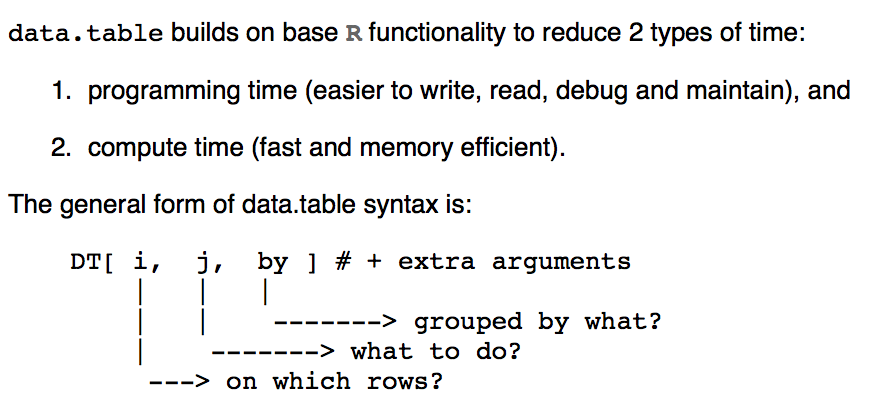
\includegraphics[scale=.5]{figures/datatable.png}
\end{center}

\end{frame}
%%%%%%%%%%%%%%%%%%%%%%%%%%%%%%%%%%%%%%%%%%%%%%%%%%%%%%%%%%%%%%%%%%%%%%%%%





%%%%%%%%%%%%%%%%%%%%%%%%%%%%%%%%%%%%%%%%%%%%%%%%%%%%%%%%%%
\begin{frame}[fragile]{\code{data.frame}s with functionality: \code{data.table}}

\begin{knitrout}\tiny
\definecolor{shadecolor}{rgb}{0.969, 0.969, 0.969}\color{fgcolor}\begin{kframe}
\begin{alltt}
\hlkwd{library}\hlstd{(data.table)}
\hlcom{#every data.table is also a data.frame}
\hlstd{DT}\hlkwb{<-}\hlkwd{data.table}\hlstd{(DF)}
\hlcom{##aggregation}
\hlstd{DT[,} \hlkwd{list}\hlstd{(}\hlkwd{mean}\hlstd{(x),} \hlkwd{sum}\hlstd{(y))]}
\end{alltt}
\begin{verbatim}
##       V1   V2
## 1: 0.216 14.9
\end{verbatim}
\end{kframe}
\end{knitrout}
\end{frame}
%%%%%%%%%%%%%%%%%%%%%%%%%%%%%%%%%%%%%%%%%%%%%%%%%%%%%%%%%%%%%%%%%%%%%%%%%



%%%%%%%%%%%%%%%%%%%%%%%%%%%%%%%%%%%%%%%%%%%%%%%%%%%%%%%%%%
\begin{frame}[fragile]{Complex Data Structures: Lists}
Lists are the most versatile data structure, allowing the collection of different lists. 
\begin{knitrout}\tiny
\definecolor{shadecolor}{rgb}{0.969, 0.969, 0.969}\color{fgcolor}\begin{kframe}
\begin{alltt}
\hlstd{LIST}\hlkwb{<-}\hlkwd{list}\hlstd{(DT, DF, letters)}

\hlkwd{class}\hlstd{(LIST)}
\end{alltt}
\begin{verbatim}
## [1] "list"
\end{verbatim}
\begin{alltt}
\hlkwd{class}\hlstd{(LIST[[}\hlnum{3}\hlstd{]])}
\end{alltt}
\begin{verbatim}
## [1] "character"
\end{verbatim}
\begin{alltt}
\hlkwd{head}\hlstd{(LIST[[}\hlnum{2}\hlstd{]])}
\end{alltt}
\begin{verbatim}
##        x      y letters
## 1  1.447 0.1562       a
## 2  0.125 0.9717       b
## 3 -0.387 0.8357       c
## 4  0.264 0.7100       d
## 5  0.434 0.0975       e
## 6 -0.942 0.2296       f
\end{verbatim}
\begin{alltt}
\hlcom{#can append items}
\hlstd{LIST[[}\hlnum{4}\hlstd{]]}\hlkwb{<-}\hlstd{y}

\hlkwd{length}\hlstd{(LIST)}
\end{alltt}
\begin{verbatim}
## [1] 4
\end{verbatim}
\end{kframe}
\end{knitrout}
\end{frame}
%%%%%%%%%%%%%%%%%%%%%%%%%%%%%%%%%%%%%%%%%%%%%%%%%%%%%%%%%%%%%%%%%%%%%%%%%


%%%%%%%%%%%%%%%%%%%%%%%%%%%%%%%%%%%%%%%%%%%%%%%%%%%%%%%%%%
\begin{frame}[fragile]{Apply functionality: vectorization}
Loops in R are inherently inefficient; most often you need to apply a function to every observation and this is where the \code{apply()} function family comes into play.

\begin{Description}
\item[base::apply] 		Apply Functions Over Array Margins
\item[base::eapply]		Apply a Function Over Values in an Environment
\item[base::lapply]		Apply a Function over a List or Vector
\item[base::mapply]		Apply a Function to Multiple List or Vector Arguments
\item[base::rapply]		Recursively Apply a Function to a List
\item[base::tapply]		Apply a Function Over a Ragged Array
\end{Description}

\end{frame}
%%%%%%%%%%%%%%%%%%%%%%%%%%%%%%%%%%%%%%%%%%%%%%%%%%%%%%%%%%%%%%%%%%%%%%%%%



%%%%%%%%%%%%%%%%%%%%%%%%%%%%%%%%%%%%%%%%%%%%%%%%%%%%%%%%%%
\begin{frame}[fragile]{Apply functionality: \code{apply}}
Returns a vector or array or list of values obtained by applying a function to margins of a matrix.

\begin{center}
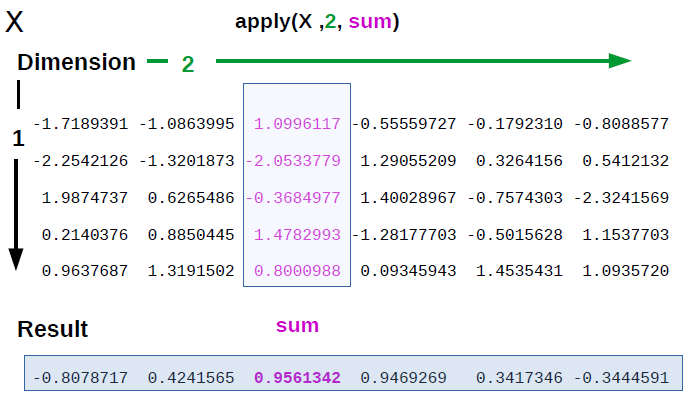
\includegraphics[scale=0.4]{figures/Apply_function.png}
\end{center}
\end{frame}
%%%%%%%%%%%%%%%%%%%%%%%%%%%%%%%%%%%%%%%%%%%%%%%%%%%%%%%%%%%%%%%%%%%%%%%%%



%%%%%%%%%%%%%%%%%%%%%%%%%%%%%%%%%%%%%%%%%%%%%%%%%%%%%%%%%%
\begin{frame}[fragile]{Apply functionality: \code{apply}}
Returns a vector or array or list of values obtained by applying a function to margins of a matrix.

\begin{knitrout}\tiny
\definecolor{shadecolor}{rgb}{0.969, 0.969, 0.969}\color{fgcolor}\begin{kframe}
\begin{alltt}
\hlcom{#create a matrix with 100 rows and 100 colums with random values drawn from uniform distribution }
\hlstd{DF}\hlkwb{<-} \hlkwd{do.call}\hlstd{(}\hlstr{"cbind"}\hlstd{,} \hlkwd{lapply}\hlstd{(}\hlnum{1}\hlopt{:}\hlnum{100}\hlstd{,} \hlkwa{function}\hlstd{(}\hlkwc{x}\hlstd{)} \hlkwd{runif}\hlstd{(}\hlkwc{n}\hlstd{=}\hlnum{100}\hlstd{)))}

\hlkwd{class}\hlstd{(DF)}
\end{alltt}
\begin{verbatim}
## [1] "matrix"
\end{verbatim}
\begin{alltt}
\hlcom{#apply function to each row: computing row sums}
\hlstd{res}\hlkwb{<-}\hlkwd{apply}\hlstd{(DF,} \hlnum{1}\hlstd{,  sum)}

\hlstd{res}
\end{alltt}
\begin{verbatim}
##   [1] 48.5 53.9 52.7 49.5 51.8 51.1 51.3 48.6 51.2 46.9 55.0 55.5 48.4 51.4 56.3 52.6 54.7
##  [18] 48.1 45.0 43.4 52.1 46.7 48.3 50.4 51.8 51.6 52.5 48.8 50.9 52.8 53.2 53.2 52.1 52.1
##  [35] 47.4 48.1 51.4 46.4 47.3 46.9 47.6 46.9 43.2 53.8 52.3 44.7 50.3 43.3 52.3 49.9 49.7
##  [52] 50.2 49.4 50.7 48.9 52.8 49.9 44.8 49.0 46.1 50.2 47.8 45.6 45.5 47.0 51.6 53.8 52.3
##  [69] 48.6 50.2 51.4 53.2 52.5 45.1 54.0 49.3 47.5 55.8 47.2 45.6 47.7 45.6 51.7 52.7 50.9
##  [86] 51.3 49.6 52.3 50.5 49.9 48.4 44.6 50.0 48.8 49.7 44.8 47.7 50.2 49.6 50.4
\end{verbatim}
\begin{alltt}
\hlkwd{rowSums}\hlstd{(DF)}
\end{alltt}
\begin{verbatim}
##   [1] 48.5 53.9 52.7 49.5 51.8 51.1 51.3 48.6 51.2 46.9 55.0 55.5 48.4 51.4 56.3 52.6 54.7
##  [18] 48.1 45.0 43.4 52.1 46.7 48.3 50.4 51.8 51.6 52.5 48.8 50.9 52.8 53.2 53.2 52.1 52.1
##  [35] 47.4 48.1 51.4 46.4 47.3 46.9 47.6 46.9 43.2 53.8 52.3 44.7 50.3 43.3 52.3 49.9 49.7
##  [52] 50.2 49.4 50.7 48.9 52.8 49.9 44.8 49.0 46.1 50.2 47.8 45.6 45.5 47.0 51.6 53.8 52.3
##  [69] 48.6 50.2 51.4 53.2 52.5 45.1 54.0 49.3 47.5 55.8 47.2 45.6 47.7 45.6 51.7 52.7 50.9
##  [86] 51.3 49.6 52.3 50.5 49.9 48.4 44.6 50.0 48.8 49.7 44.8 47.7 50.2 49.6 50.4
\end{verbatim}
\begin{alltt}
\hlkwd{sum}\hlstd{(res}\hlopt{!=}\hlkwd{rowSums}\hlstd{(DF))}
\end{alltt}
\begin{verbatim}
## [1] 0
\end{verbatim}
\begin{alltt}
\hlcom{#apply function to each column: computing column sums}
\hlstd{res}\hlkwb{<-}\hlkwd{apply}\hlstd{(DF,} \hlnum{2}\hlstd{,  sum)}

\hlstd{res}
\end{alltt}
\begin{verbatim}
##   [1] 50.8 50.5 48.9 52.7 48.8 48.7 47.8 49.0 49.0 50.5 52.1 43.3 51.8 50.0 53.1 47.0 49.3
##  [18] 46.0 55.0 49.4 52.9 53.8 49.7 52.8 47.7 51.1 49.4 55.1 52.5 52.0 49.1 49.0 46.2 44.9
##  [35] 53.2 52.8 49.0 47.6 44.9 51.5 46.2 48.6 46.0 49.1 45.9 53.2 48.3 48.8 51.8 53.4 46.8
##  [52] 45.2 49.2 47.2 50.9 50.0 50.3 52.7 49.0 53.0 53.7 50.9 54.1 53.6 49.0 48.8 49.2 44.4
##  [69] 52.6 54.5 46.9 45.3 45.0 54.9 50.8 50.0 51.0 54.4 47.5 48.6 47.9 51.2 48.4 50.1 46.7
##  [86] 47.9 51.0 45.7 49.5 48.4 48.0 50.1 53.4 50.6 52.3 50.0 52.2 47.4 43.5 53.1
\end{verbatim}
\begin{alltt}
\hlkwd{colSums}\hlstd{(DF)}
\end{alltt}
\begin{verbatim}
##   [1] 50.8 50.5 48.9 52.7 48.8 48.7 47.8 49.0 49.0 50.5 52.1 43.3 51.8 50.0 53.1 47.0 49.3
##  [18] 46.0 55.0 49.4 52.9 53.8 49.7 52.8 47.7 51.1 49.4 55.1 52.5 52.0 49.1 49.0 46.2 44.9
##  [35] 53.2 52.8 49.0 47.6 44.9 51.5 46.2 48.6 46.0 49.1 45.9 53.2 48.3 48.8 51.8 53.4 46.8
##  [52] 45.2 49.2 47.2 50.9 50.0 50.3 52.7 49.0 53.0 53.7 50.9 54.1 53.6 49.0 48.8 49.2 44.4
##  [69] 52.6 54.5 46.9 45.3 45.0 54.9 50.8 50.0 51.0 54.4 47.5 48.6 47.9 51.2 48.4 50.1 46.7
##  [86] 47.9 51.0 45.7 49.5 48.4 48.0 50.1 53.4 50.6 52.3 50.0 52.2 47.4 43.5 53.1
\end{verbatim}
\begin{alltt}
\hlkwd{sum}\hlstd{(res}\hlopt{!=}\hlkwd{colSums}\hlstd{(DF))}
\end{alltt}
\begin{verbatim}
## [1] 0
\end{verbatim}
\end{kframe}
\end{knitrout}
\end{frame}
%%%%%%%%%%%%%%%%%%%%%%%%%%%%%%%%%%%%%%%%%%%%%%%%%%%%%%%%%%%%%%%%%%%%%%%%%


%%%%%%%%%%%%%%%%%%%%%%%%%%%%%%%%%%%%%%%%%%%%%%%%%%%%%%%%%%
\begin{frame}[fragile]{Apply functionality: \code{lapply}}
\code{lapply} returns a list of the same length as X, each element of which is the result of applying FUN to the corresponding element of X.

\begin{knitrout}\tiny
\definecolor{shadecolor}{rgb}{0.969, 0.969, 0.969}\color{fgcolor}\begin{kframe}
\begin{alltt}
\hlcom{#apply any function on a vector, returns a list}
\hlstd{res}\hlkwb{<-}\hlkwd{lapply}\hlstd{(}\hlnum{1}\hlopt{:}\hlnum{1000}\hlstd{,} \hlkwa{function}\hlstd{(}\hlkwc{x}\hlstd{) x}\hlopt{^}\hlnum{0.5}\hlstd{)}

\hlkwd{class}\hlstd{(res)}
\end{alltt}
\begin{verbatim}
## [1] "list"
\end{verbatim}
\begin{alltt}
\hlkwd{head}\hlstd{(}\hlkwd{unlist}\hlstd{(res))}
\end{alltt}
\begin{verbatim}
## [1] 1.00 1.41 1.73 2.00 2.24 2.45
\end{verbatim}
\end{kframe}
\end{knitrout}

``sapply is a user-friendly version of lapply by default returning a vector or matrix if appropriate.``
\end{frame}
%%%%%%%%%%%%%%%%%%%%%%%%%%%%%%%%%%%%%%%%%%%%%%%%%%%%%%%%%%%%%%%%%%%%%%%%%



%%%%%%%%%%%%%%%%%%%%%%%%%%%%%%%%%%%%%%%%%%%%%%%%%%%%%%%%%%
\begin{frame}[fragile]{Basic Plots}
\code{R} has amazing plotting functionality, beyond the scope of this course to go in too much detail. Base-R provides simple plotting functionality, advanced and fancy plots are possible with the ggplot package.

Base-R tries to guess the appropriate plotting function dependent on the data type.
\begin{knitrout}\tiny
\definecolor{shadecolor}{rgb}{0.969, 0.969, 0.969}\color{fgcolor}\begin{kframe}
\begin{alltt}
\hlstd{x}\hlkwb{<-}\hlkwd{rnorm}\hlstd{(}\hlkwc{n}\hlstd{=}\hlnum{26}\hlstd{)}
\hlstd{y}\hlkwb{<-}\hlkwd{runif}\hlstd{(}\hlkwc{n}\hlstd{=}\hlnum{26}\hlstd{)}
\hlstd{DF}\hlkwb{<-}\hlkwd{data.frame}\hlstd{(x,y,}\hlstr{"letters"}\hlstd{=}\hlkwd{sample}\hlstd{(letters[}\hlnum{1}\hlopt{:}\hlnum{4}\hlstd{],}\hlnum{26}\hlstd{,} \hlkwc{replace}\hlstd{=}\hlnum{TRUE}\hlstd{))}
\hlcom{#simple scatter plot}
\hlkwd{plot}\hlstd{(DF}\hlopt{$}\hlstd{x,DF}\hlopt{$}\hlstd{y,} \hlkwc{col}\hlstd{=DF}\hlopt{$}\hlstd{letters)}
\end{alltt}
\end{kframe}

{\centering 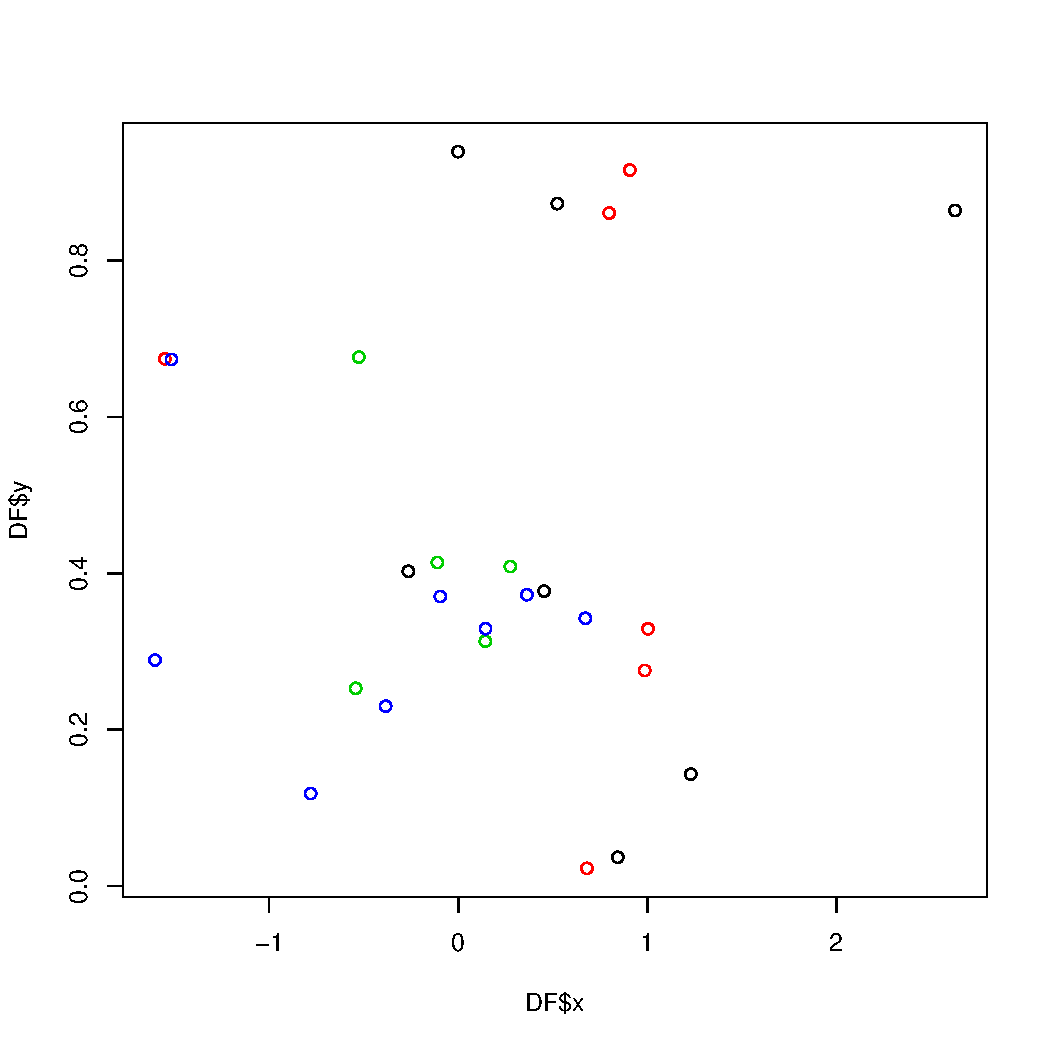
\includegraphics[width=2in]{figures/knitr-plots1-1} 

}



\end{knitrout}
\end{frame}
%%%%%%%%%%%%%%%%%%%%%%%%%%%%%%%%%%%%%%%%%%%%%%%%%%%%%%%%%%%%%%%%%%%%%%%%%



%%%%%%%%%%%%%%%%%%%%%%%%%%%%%%%%%%%%%%%%%%%%%%%%%%%%%%%%%%
\begin{frame}[fragile]{Basic Plots}
\begin{knitrout}\tiny
\definecolor{shadecolor}{rgb}{0.969, 0.969, 0.969}\color{fgcolor}\begin{kframe}
\begin{alltt}
\hlcom{#letters is a factor (an encoded string), so appropriate is to draw a boxplot}
\hlkwd{plot}\hlstd{(DF}\hlopt{$}\hlstd{letters,DF}\hlopt{$}\hlstd{y)}
\end{alltt}
\end{kframe}

{\centering 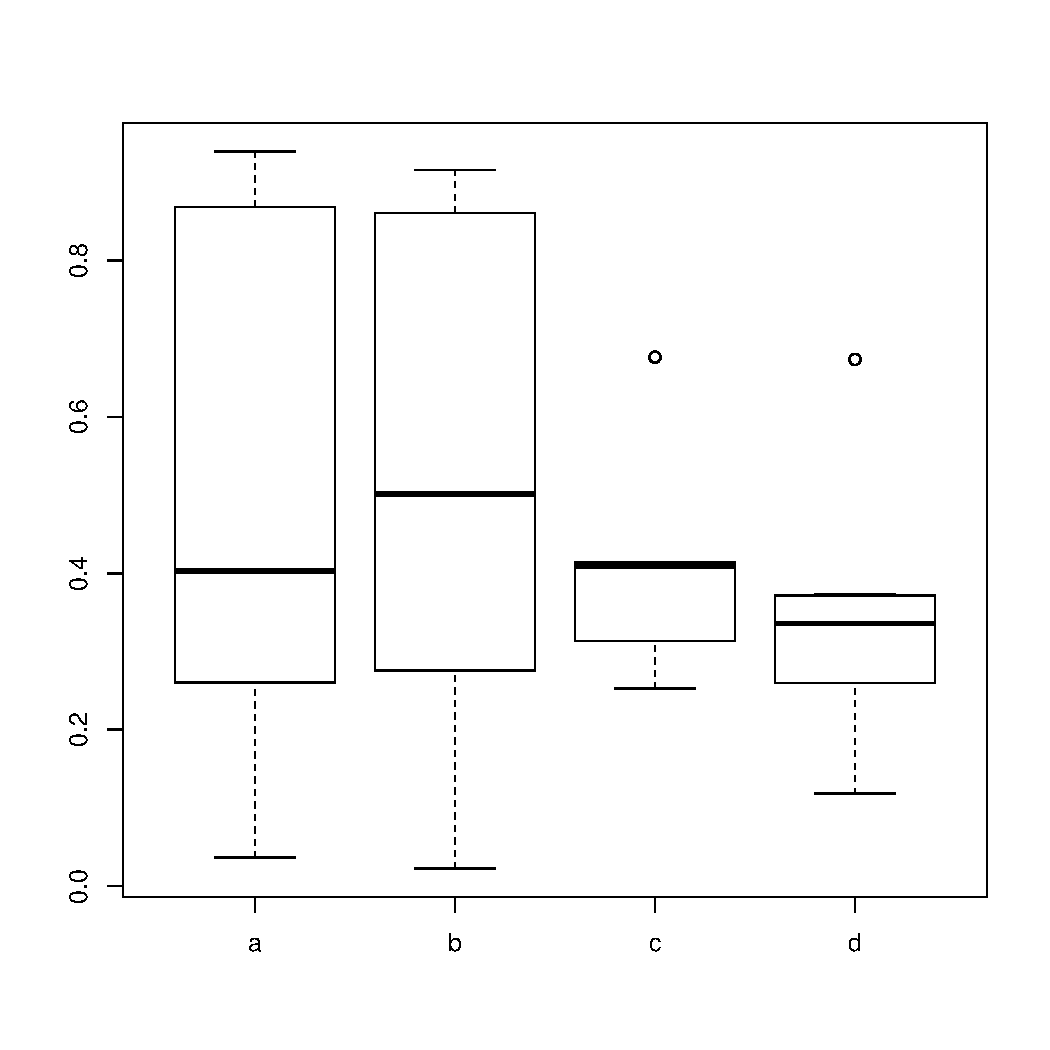
\includegraphics[width=2in]{figures/knitr-plots2-1} 

}



\end{knitrout}
\end{frame}
%%%%%%%%%%%%%%%%%%%%%%%%%%%%%%%%%%%%%%%%%%%%%%%%%%%%%%%%%%%%%%%%%%%%%%%%%




%%%%%%%%%%%%%%%%%%%%%%%%%%%%%%%%%%%%%%%%%%%%%%%%%%%%%%%%%%
\begin{frame}[fragile]{Basic Plots}
\begin{knitrout}\tiny
\definecolor{shadecolor}{rgb}{0.969, 0.969, 0.969}\color{fgcolor}\begin{kframe}
\begin{alltt}
\hlcom{#kernel density}
\hlkwd{plot}\hlstd{(}\hlkwd{density}\hlstd{(DF}\hlopt{$}\hlstd{x))}
\end{alltt}
\end{kframe}

{\centering 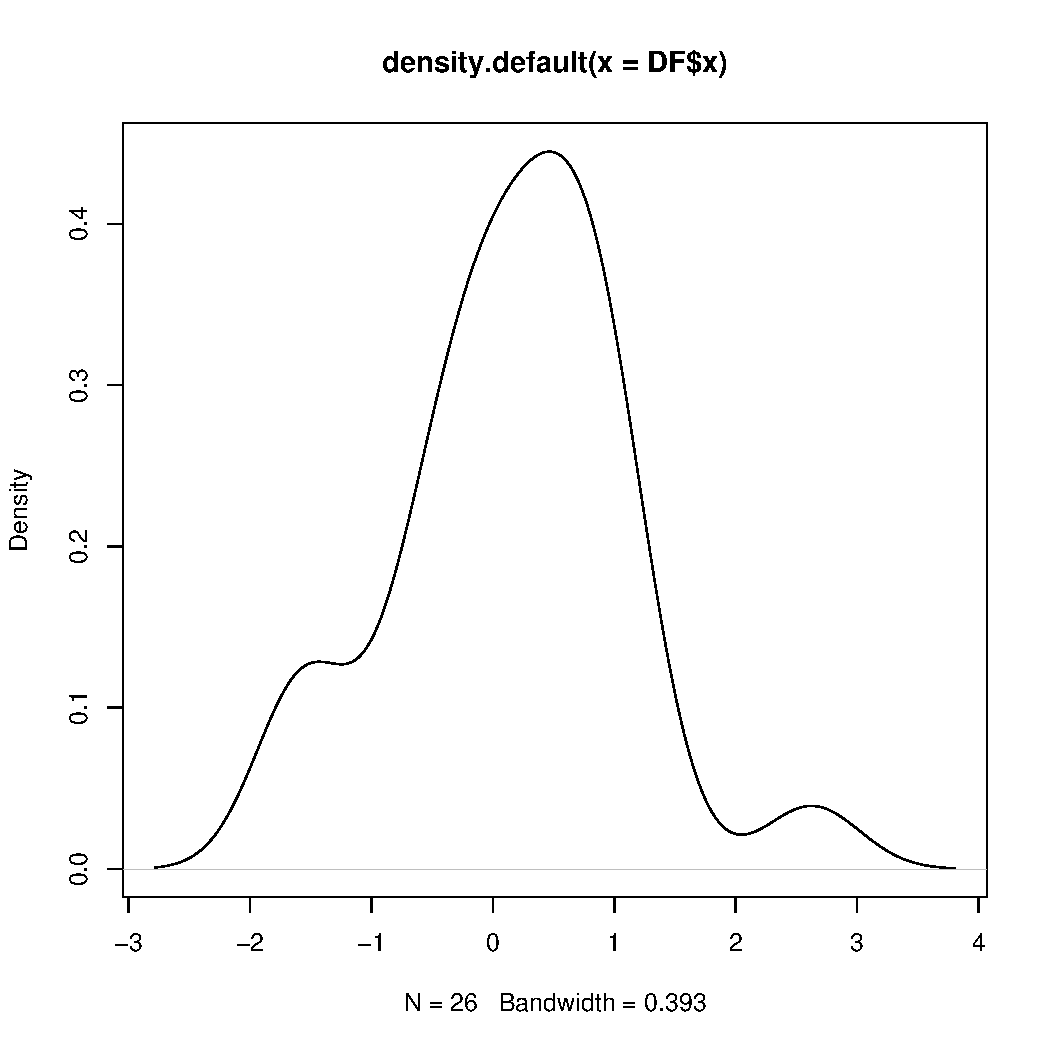
\includegraphics[width=2in]{figures/knitr-plots3-1} 

}



\end{knitrout}
\end{frame}
%%%%%%%%%%%%%%%%%%%%%%%%%%%%%%%%%%%%%%%%%%%%%%%%%%%%%%%%%%%%%%%%%%%%%%%%%



%%%%%%%%%%%%%%%%%%%%%%%%%%%%%%%%%%%%%%%%%%%%%%%%%%%%%%%%%%
\begin{frame}[fragile]{Basic Plots}
\begin{knitrout}\tiny
\definecolor{shadecolor}{rgb}{0.969, 0.969, 0.969}\color{fgcolor}\begin{kframe}
\begin{alltt}
\hlcom{#histogram}
\hlkwd{hist}\hlstd{(DF}\hlopt{$}\hlstd{x)}
\end{alltt}
\end{kframe}

{\centering 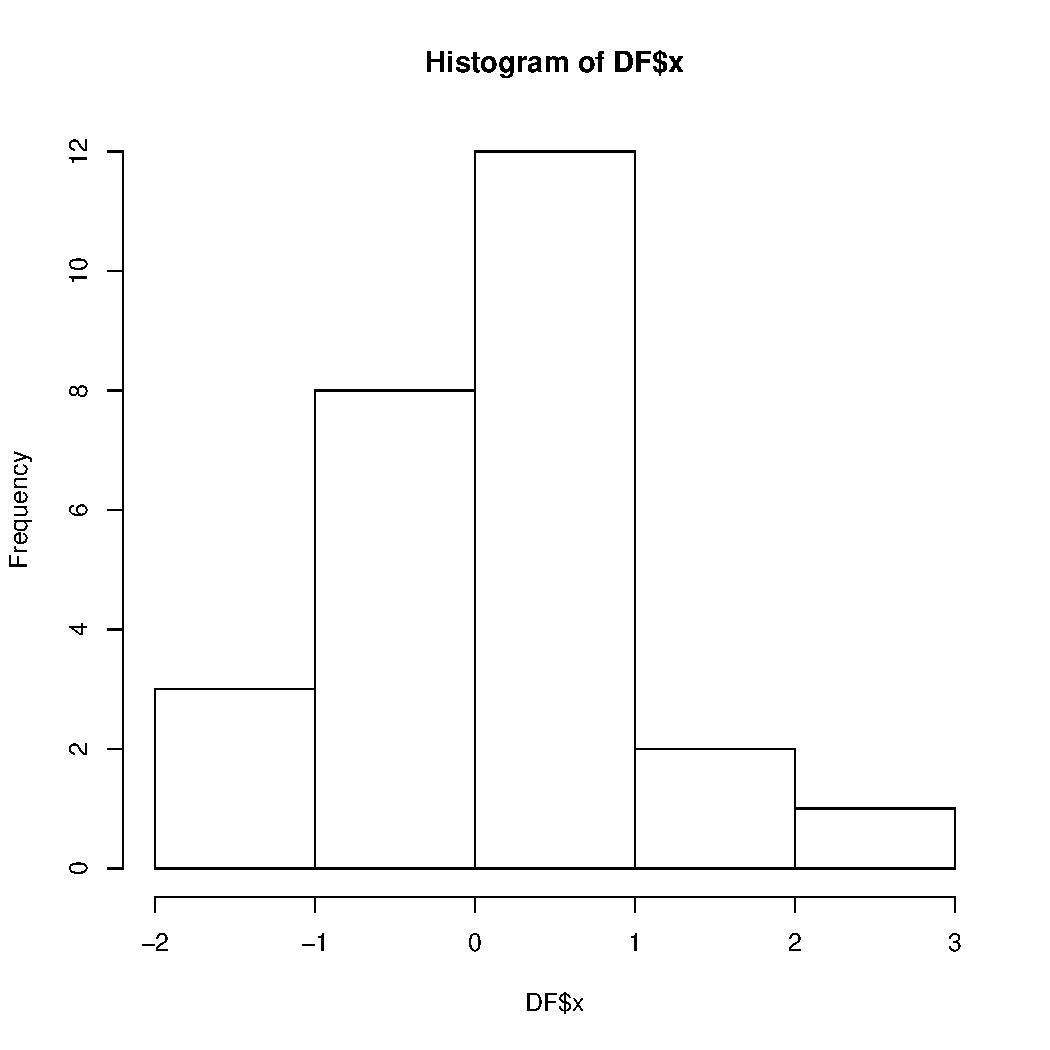
\includegraphics[width=2in]{figures/knitr-plots4-1} 

}



\end{knitrout}
\end{frame}
%%%%%%%%%%%%%%%%%%%%%%%%%%%%%%%%%%%%%%%%%%%%%%%%%%%%%%%%%%%%%%%%%%%%%%%%%


%%%%%%%%%%%%%%%%%%%%%%%%%%%%%%%%%%%%%%%%%%%%%%%%%%%%%%%%%%
\begin{frame}[fragile]{A Texteditor is very very useful...}

\begin{itemize}
\item Textwranger (Mac), Notepad++ (Windows), or system text editor (Windows Editor / Mac Text.app)

\item Very good to look at raw text in editor before loading into R to see how messy it is.

\item Especially machine read data (PDFs processed with Optical Character recognition - OCR)
\begin{figure}[h]
\begin{center}
\includegraphics[scale=.2]<1>{figures/textwrangler.jpeg}
\includegraphics[scale=.2]<1>{figures/notepadpp.png}
\includegraphics[scale=.2]<1>{figures/windowseditor.jpeg}
\includegraphics[scale=.2]<2>{figures/messier}
\includegraphics[scale=.2]<3>{figures/messy}
\end{center}
%\caption{\small{EU Enlargement in 2004}}
\end{figure}

\end{itemize}

\end{frame}
%%%%%%%%%%%%%%%%%%%%%%%%%%%%%%%%%%%%%%%%%%%%%%%%%%%%%%%%%%%%%%%%%%%%%%%%%

%%%%%%%%%%%%%%%%%%%%%%%%%%%%%%%%%%%%%%%%%%%%%%%%%%%%%%%%%%
\begin{frame}[fragile]{Text Encoding: A cautionary note}

\begin{itemize}
\item Especially working with data from different computer systems (Mac, Unix, Windows) and different languages, character encoding issues can occur.
\item The Latin character set (Encoding: \code{latin-1}) is used by English and most European languages, though the Greek character set is used only by the Greek language.

\item Loading data without knowing character encoding can sometimes cause errors

\item Text editors like Textwranger attempt to recognize character encoding

\item Most common encoding is \code{UTF-8}
\end{itemize}

\begin{figure}[h]
\begin{center}
\includegraphics[scale=.5]<1>{figures/invalid-multibyte}
\end{center}
%\caption{\small{EU Enlargement in 2004}}
\end{figure}


\end{frame}
%%%%%%%%%%%%%%%%%%%%%%%%%%%%%%%%%%%%%%%%%%%%%%%%%%%%%%%%%%%%%%%%%%%%%%%%%





\end{document}

